\documentclass[11pt,letterpaper]{article}
\usepackage{graphicx,amsmath,amsthm,amsfonts,amssymb,fullpage,xcolor,tikz,pgfplots,multirow,multicol,hyperref,caption, geometry,float,bbold}
\geometry{margin=1in}
\usepackage{setspace}
\setstretch{1.2}
\usepackage{enumerate}
\usepackage{graphicx}
\usepackage{caption}
\usepackage[operators,sets]{cryptocode}
\usepackage{authblk} % for affiliations
\usepackage{draftwatermark}

% Customize the watermark
\SetWatermarkText{DRAFT}          % The watermark text
\SetWatermarkScale{5}             % Size (increase for full-page)
\SetWatermarkColor[gray]{0.85}    % Light gray
\SetWatermarkAngle{45}            % Diagonal placement
\SetWatermarkFontSize{5cm}        % Optional: explicit size
\SetWatermarkLightness{0.9}       % Optional: even lighter
\SetWatermarkHorCenter{0.5\paperwidth} % Optional: repositioning
\SetWatermarkVerCenter{0.5\paperheight}

\newtheorem{thm}{Theorem}[section]
\newtheorem{ex}{Example}[section]

\newcommand{\polys}{K[X,Y]}
\newcommand{\hpolys}{K[X\!:\!Y\!:\!Z]}
\newcommand{\productpolys}{K[X_1, Y_1, \ldots, X_n, Y_n]}


\newcommand{\dX}{\frac{\partial}{\partial X}}
\newcommand{\dY}{\frac{\partial}{\partial Y}}
\newcommand{\dXP}{\frac{\partial}{\partial X_P}}
\newcommand{\dYP}{\frac{\partial}{\partial Y_P}}
\newcommand{\dXQ}{\frac{\partial}{\partial X_Q}}
\newcommand{\dYQ}{\frac{\partial}{\partial Y_Q}}
\newcommand{\dZ}{\frac{\partial}{\partial Z}}

\newcommand{\free}[1]{{\textcolor{red}{#1}}}
\newcommand{\luke}[1]{{\textcolor{purple}{#1}}}
\newcommand{\rigo}[1]{{\textcolor{blue}{#1}}}
\newcommand{\brando}[1]{{\textcolor{green}{#1}}}




%%% Freeman's Macros %%%
\theoremstyle{definition}
\newtheorem{proposition}{Proposition}
\newtheorem{theorem}{Theorem}
\newtheorem{definition}{Definition}
\newtheorem{remark}{Remark}
\newtheorem{problem}{Problem}
\newtheorem{lemm}{Lemma}[section]
\newtheorem{defn}{Definition}

\def\do#1{\csdef{#1}{\mathbb{#1}}}
\docsvlist{N,A,P,Z,Q,G,H}
\def\do#1{\csdef{#1}{\mathcal{#1}}}
\docsvlist{E,M,R,C,S,F,V,R,W,S,L,B,O}

\newcommand{\ff}{K(\E)}

\pgfplotsset{compat=1.18}
\setlength\parindent{1.5em}

\newcommand{\Fq}{\mathbb{F}_q}
\newcommand{\Fqm}{\mathbb{F}_{q^m}}
\newcommand{\Fqn}{\mathbb{F}_{q}^n}
\newcommand{\Fqmn}{\mathbb{F}_{q^m}^n}
\newcommand{\Fp}{\mathbb{F}_p}
\newcommand{\Fpn}{\mathbb{F}_{p}^n}
\newcommand{\6}{\mathbf}
\newcommand{\7}{\mathcal}
\newcommand{\rar}{\rightarrow}
\newcommand{\lar}{\leftarrow}
\newcommand{\lsamp}{\xleftarrow{\$}}
\newcommand{\map}{\mapsto}
\newcommand{\til}[1]{{\tilde{#1}}}
\newcommand{\hsh}[1]{\text{Hash}{(#1)}}
\renewcommand\epsilon\varepsilon
\newcommand{\ip}[2]{{\langle {#1}, \, {#2} \rangle}}
\newcommand{\dimFp}[1]{{\text{dim}_{\mathbb{F}_p}(#1)}}

\newcommand{\com}[1]{{\mathsf{commit}(#1)}}


\newcommand{\divi}[1]{{\text{div}(#1)}}
\newcommand{\lr}[1]{{\langle #1 \rangle}}

\captionsetup[table]{name = Algorithm}


\newcommand{\zon}{\{0, \, 1\}^n}
\newcommand{\zo}{\{0, \, 1\}}
\newcommand{\one}{\mathbb{1}}
\newcommand{\zero}{\mathbb{0}}








\title{
SLVer Bullet: \underline{S}traight-\underline{L}ine \underline{Ver}ification for \underline{Bullet}proofs
}
\author{Brandon Goodell, Rigo Salazar, Freeman Slaughter, Luke Szramowski
}
\affil{$\mathsf{Cypher \ Stack}$}

\date{\today}




\begin{document}

\maketitle

\section*{Disclaimer}

This paper is not yet completed; future updates to this document are forthcoming soon.

\section{Introduction}


In \cite{Eagen}, Eagen proposed a method for checking whether a sum of points in an elliptic curve group has been computed correctly. The approach offloads computational costs faced by verifiers to provers, which is useful when verification must be performed repeatedly.
Although the iterative witness construction algorithm proposed in \cite{Eagen} is correct, \cite{Eagen} is rather informal, lacking formal protocol descriptions, claims, proofs, or efficiency analyses. In \cite{Kayaba}, Parker used Eagen's method  in rank-$1$ constraint systems to verify  scalar multiplication of group elements, proposing a protocol based on Eagen's arguments. In \cite{SoundnessForDLP}, Bassa contributed towards formalizing Eagen's method, explicitly describing Parker's proof of scalar multiplication and sketching arguments towards proofs of soundness.

% We expressly compute the completeness and soundness error for this approach, because, while welcome, we do not believe that Bassa's analysis was without errors.
% We then apply this approach to zero-knowledge proof systems to highlight the computational advantage offered by divisors, offloading the bulk of the computational bottleneck on the verifier's side to the prover.
% In particular, we implement the divisors framework with the Schnorr scheme and Bulletproofs, as they are most applicable to cryptocurrencies such as Monero or Salvium, though note that these are not the only protocols who may benefit from this perspective.



% We formalize a divisors-based modification to an existing proof-of-computation scheme. The original scheme, described first publicly by Eagen in \cite{Eagen}, checks whether a sum of points in some elliptic curve group $\G$ defined over a finite field $K$ has been computed correctly, using only linear combinations over $K$. The approach allows for pre-computation, so that users of a zero-knowledge proving scheme may optionally offload computational cost from verifiers to provers.
% In \cite{Kayaba}
% This approach was utilized in Parker \cite{Kayaba} for proving group point relationships within rank $1$ constraint systems. 


However, the soundness arguments in \cite{SoundnessForDLP} are not without  obstacles. In \cite{Eagen}, rational solutions to certain systems of polynomial equations are assumed to exist.
Unfortunately, these equations do not admit such solutions in general, so the verification equations proposed in \cite{Eagen} and studied in \cite{SoundnessForDLP} are not justified. Bassa lifted to the surface of pairs of elliptic curve group points, partially resolving the problem. 

Bassa's approach implies changes to the verification equations  of \cite{Eagen}, however. We formalize the correct verification equations, and consider the security of Eagen's approach. We present a corrected version of the general protocol, and explicitly compute the completeness and soundness errors.
We show how our corrected scheme can be used to verify scalar multiplication as in Parker's proposed protocol.
We then apply this approach to zero-knowledge proof systems to illustrate the computational advantage offered by divisors. 
In particular, the prover can pre-compute division operations for the verifier, which are the computational bottlenecks on the verifier's side.
In particular, we transform the interactive Schnorr identification protocol \cite{Schnorr} and an interactive Bulletproofs range-proving protocol \cite{Bullet}, and benchmark efficiency.
We choose Schnorr and Bulletproofs because these protocols are simple, secure, popular, and readily applicable in cryptocurrencies such as Monero or Salvium.  
% The efficiency gains here are most applicable to currencies such as Monero or Salvium, though note that these are not the only protocols who may benefit from this perspective,


% We expand upon Bassa's work in \cite{SoundnessForDLP} by presenting a corrected version of Bassa's protocol, and explicitly computing the completeness and soundness error.
% We exemplify the approach with a simple, non-zero-knowledge proof of scalar multiplication.
% We then transform zero-knowledge proof systems, allowing provers to pre-compute data for verifiers, such that verification is a straight-line program with computations over the base field. 
% This offloads the bulk of the computational cost faced by verifiers to the prover.
% The transformation is somewhat general, but we exemplify the approach with a transformed Schnorr identification protocol and a transformed range proving system via bulletproofs. The Schnorr and bulletproofs protocols  are simple, secure, popular, and applicable (as in cryptocurrencies like Monero or Salvium), so they make for good demonstrations. We then analyze the efficiency of the approach against the un-transformed versions of these protocols.

\subsection{Change log}

This document will be updated occasionally, especially when security-sensitive results come to light. We summarize such changes here.
\begin{itemize}
\item 11 June 2025. Initial preprint.
\end{itemize}


\section{Notation and preliminary definitions}

We begin assuming the reader has knowledge of basic algebra concepts related to groups, rings, and fields. Our notation and background primarily follows \cite{Silverman}, but we depart notationally in a few notable ways, especially with regard to divisors.

\subsection{Polynomials and rational functions}

For a set $S$, we use $x \lsamp S$ to mean that the element $x$ was sampled uniformly at random from set $S$.
Let $\one$ and $\zero$ be the vectors of all $1$'s and $0$'s, respectively.
If $R$ is a ring, we write $R^\times = R\setminus\left\{0\right\}$ to denote the multiplicative subgroup. 
Let $p$ be a prime, $K$ a finite field with $\text{char}(K) = p$, algebraic closure $\overline{K}$, and multiplicative subgroup $K^\times = \left\{x \in K \mid x \neq 0\right\}$. Let $X, Y, Z$ be indeterminates over $\overline{K}$. Finite linear combinations in products of $X$, $Y$, and $Z$ are \textit{polynomials}. We use the following usual notation for rings of polynomials over $\overline{K}$ and $K$.
\begin{itemize}

\item  $\overline{K}[X,Y] = \left\{\sum_{i=0}^{n}\sum_{j=0}^{m} a_{i,j} X^i Y^j \mid a_{i,j} \in \overline{K}\right\}$

\item $\polys = \left\{\sum_{i=0}^{n}\sum_{j=0}^{m}a_{ij} X^iY^j \mid a_{ij} \in K\right\}$

\item  $\overline{K}[X,Y,Z] = \left\{\sum_{i=0}^{n}\sum_{j=0}^{m} \sum_{k=0}^{l} a_{i,j,k} X^i Y^j Z^l \mid a_{i,j,l} \in \overline{K}\right\}$

\item $K[X,Y,Z] = \left\{\sum_{i=0}^{n}\sum_{j=0}^{m} \sum_{k=0}^{l} a_{i,j,k} X^i Y^j Z^l \mid a_{i,j,l} \in K\right\}$

\end{itemize}  

For $f = \sum_i \sum_j a_{ij} X^iY^j \in \polys$, define $\text{deg}(f) = \max \left\{i+j \mid a_{ij} \neq 0\right\}$ (and similarly for the other polynomial rings). Each of these rings admits a structure-preserving map $\text{deg}:R \to \N_0 = \N \cup \left\{0\right\}$ such that $\text{deg}(fg) = \text{deg}(f) + \text{deg}(g)$, $\text{deg}(f+g) \leq \max\left\{\text{deg}(f), \text{deg}(g)\right\}$. Also, $\text{deg}(f) = 0$ if and only if $f = 0$.

We also define the respective field extensions of rational functions $\overline{K}(X,Y)$, $K(X,Y)$, $\overline{K}(X,Y,Z)$, and $K(X,Y,Z)$ as usual. Given $P = (x,y) \in \overline{K}^2$, the following is a well-defined map on rational functions $f \in \overline{K}(X,Y)$.
\begin{align}
\text{ord}_P(f) =& \begin{cases} m > 0; & P\text{ is a root of }f\text{ with multiplicity }m \\ m < 0; & P\text{ is a pole of }f\text{ with multiplicity }\left|m\right|=-m \\ 0; & \text{otherwise} \end{cases}
\end{align} We define $\text{ord}_P(f)$ similarly for $f \in K(X,Y)$.

If $d, n \in \mathbb{N}_0$ and $f = \sum_{ij} a_{ij}X^iY^j$ has some $\lambda \in K^\times$ such that $f(\lambda X, \lambda Y) = \lambda^d f(X,Y)$, then we say $f$ is \textit{homogeneous with degree} $d$; otherwise, \textit{inhomogeneous}. Define an equivalence relation on the subset of homogeneous polynomials in $K[X,Y,Z]$ such that every $f(X,Y,Z) \in K[X,Y,Z]$ relates to $f(\lambda X, \lambda Y, \lambda Z)$ for every $\lambda \in K^\times$. Denote the equivalence class of $f$ under this equivalence relation with $f(X\!:\!Y\!:\!Z)$, and the set of equivalence classes under this relation with $K[X\!:\!Y\!:\!Z]$. Similarly define $\overline{K}[X\!:\!Y\!:\!Z]$.
Define $\text{deg}:\overline{K}[X:Y:Z] \to \N_0$ by declaring $\text{deg}(f(X\!:\!Y\!:\!Z)) = \text{deg}(f(X,Y,Z))$. Similarly define $K[X\!:\!Y\!:\!Z]$ and its degree function. The rings $\overline{K}[X,Y]$, $K[X,Y]$, $\overline{K}[X,Y,Z]$, $K[X,Y,Z]$, $\overline{K}[X\!:\!Y\!:\!Z]$, and $K[X\!:\!Y\!:\!Z]$ are all integral domains. 

In the sequel, we use the distinguished family of polynomials parameterized by $\alpha, \beta \in K^2$ of the form $e = Y^2 - X^3 - \alpha X - \beta \in K[X,Y]$ such that $4\alpha^3 + 27\beta^2 \neq 0$; these are exactly the non-singular elliptic curves.

\subsection{Affine and projective planes}

Define $\A^2(\overline{K}) = \left\{(x,y) \in \overline{K}^2\right\}$, $\A^3(\overline{K}) = \left\{(x,y,z) \in \overline{K}^3\right\}$, $\A^2(K) = \left\{(x,y) \in K^2\right\}$, and $\A^3(K)=\left\{(x,y,z) \in K^3\right\}$.  We say the elements of $\mathbb{A}^2(\overline{K})$ are \textit{affine points} and the elements of $\mathbb{A}^2(K)$ are \textit{$K$-rational} affine points. 
For any ideal $I \subseteq \overline{K}[X,Y]$, the \textit{affine vanishing set} of $I$ is  $v_a(I) = \left\{(x,y) \in \mathbb{A}^2(\overline{K}) \mid f(x,y) = 0\text{ for all } f \in I\right\}$. If $f(X,Y) \in \overline{K}[X,Y]$, we define the affine vanishing set for $f$ as the affine vanishing set for the principally generated $I = (f)$, which we denote with $v_a(f)$.


Given affine vanishing set $V$, let $I(V) = \left\{f \in \overline{K}[X,Y] \mid f(x,y) = 0\text{ for all }(x,y) \in V\right\}$  be the \textit{ideal of $V$}. It is easy to check that $I(V)$ is an ideal of $\overline{K}[X,Y]$.
We say an affine vanishing set $V$ is \textit{defined over} $K$, denoted with shorthand $V/K$, if $I(V)$ is generated as an ideal in $\overline{K}[X,Y]$ by a subset of $K[X,Y]$. 
For any affine vanishing set $V$, let $I(V/K) = \left\{f \in \polys \mid f(x,y) = 0\text{ for all }(x,y) \in V\right\} = I(V) \cap K[X,Y]$. It is easy to show that $I(V/K)$ is an ideal. Moreover, $V$ is defined over $K$ if and only if $I(V)$ is generated as an ideal in $\overline{K}[X,Y]$ by $I(V/K)$, i.e.\ $I(V) = I(V/K)\overline{K}[X,Y]$. 

We say $V$ is an \textit{affine variety} if $I(V)$ is a prime ideal in $\overline{K}[X,Y]$. The \textit{affine coordinate ring} of an affine variety $V/K$ is the quotient ring $K[V] = \frac{K[X,Y]}{I(V/K)}$. The \textit{function field} of $V$ is the field of fractions $K(V)$ associated with $K[V]$, i.e.\ the set of all formal fractions $\frac{f}{g}$ where $f, g \in K[V]$ and $g \neq 0$, under an equivalence relation defined by relating $\frac{f_1}{g_1}$ to $\frac{f_2}{g_2}$ if and only if $f_1 g_2 - f_2 g_1 = 0$.

Define an equivalence relation on $\A^3(\overline{K}) \setminus \left\{\zero\right\}$ by relating $(x,y,z)$ to $(x^\prime, y^\prime, z^\prime)$ if and only if there exists $\lambda \in \overline{K}^\times$ such that $(x^\prime, y^\prime, z^\prime) = (\lambda x, \lambda y, \lambda z)$. Use $\P^2(\overline{K})$ to denote the set of equivalence classes under this relation. Similarly define $\P^2(K)$ in the evident way. We say the elements of $\P^2(\overline{K})$ are \textit{projective points} and the elements of $\P^2(K)$ are the \textit{$K$-rational} projective points. For any homogeneous ideal $I \subseteq \overline{K}[X,Y,Z]$, the \textit{projective vanishing set} of $I$ is $v_p(I) = \left\{(x\!:\!y\!:\!z) \in \P^2(\overline{K}) \mid f(x,y,z)=0\text{ for all }f \in I\right\}$. Since the generating set for $I$ contains only homogeneous polynomials, the presence of any representative in $(x\!:\!y\!:\!z)$ which kills $f$ implies all representatives kill $f$. For any $f \in \overline{K}[X,Y,Z]$, we define the projective vanishing set for $f$ as the projective vanishing set for the ideal $I=(f)$, and we use the notation $v_p(f)$.



Given a projective vanishing set $V$, we overload notation and define $I(V)$ to be the homogeneous ideal of $\overline{K}[X\!:\!Y\!:\!Z]$ generated by the set $\left\{f \in \overline{K}[X\!:\!Y\!:\!Z] \mid f(x\!:\!y\!:\!z) = 0\text{ for all }(x\!:\!y\!:\!z) \in V\right\}$.
We say a projective vanishing set $V$ is \textit{defined over} $K$, denoted with shorthand $V/K$, if $I(V)$ is generated as an ideal in $\overline{K}[X\!:\!Y\!:\!Z]$ by a subset of $K[X\!:\!Y\!:\!Z]$. 
We say $V$ is a \textit{projective variety} if its homogeneous ideal $I(V)$ is a prime ideal in $\overline{K}[X,Y,Z]$. The \textit{projective coordinate ring} of an projective variety $V/K$ is the quotient ring $K[V] = \frac{K[X\!:\!Y\!:\!Z]}{I(V/K)}$. %The \textit{function field} of $V$ is the field of fractions $K(V)$, i.e.\ the set of all formal fractions $\frac{f}{g}$ where $f, g \in K[V]$ and $g \neq 0$, under an equivalence relation defined by relating $\frac{f_1}{g_1}$ to $\frac{f_2}{g_2}$ if and only if $f_1 g_2 - f_2 g_1 = 0$.


Affine points $P=(x,y) \in \A^2(\overline{K})$ naturally map to projective points $P^*=(x:y:1) \in \P^2(\overline{K})$. This map is injective. Projective points $P=(x\!:\!y\!:\!z) \in \P^2(\overline{K})$ with $z \neq 0$ naturally map to affine points $P_*=(\frac{x}{z}, \frac{y}{z}) \in \A^2(\overline{K})$ in a similar way, but surjectively. The same statement as above holds with $\A^2(K)$ and $\P^2(K)$ replacing their counterparts everywhere.

There exists natural \textit{homogenization} maps carrying $f \in \polys$ (or $f \in \overline{K}[X,Y]$) to a homogeneous $f^* \in K[X,Y,Z]$ (or $f^* \in \overline{K}[X,Y,Z]$, respectively) where $f^* = Z^{\text{deg}(f)}f(\frac{X}{Z}, \frac{Y}{Z})$. This map is injective.
We can also dehomogenize a homogeneous polynomial $g \in \hpolys$ (or $\overline{K}[X,Y,Z]$) to a polynomial in the affine coordinate ring $g \mapsto g_*(X,Y) = g(X:Y:1) \in \polys$ (or $\overline{K}[X,Y]$, respectively). This map is surjective.

Using these maps, we can make sense of embedding $\A^2$ in $\P^2$, and projecting $\P^2$ back to $\A^2$.  In this way, we define \textit{projective closure} of an affine variety $V$ as the projective vanishing set $\overline{V}$ such that $I(\overline{V}) = \left\{f^* \mid f \in I(V)\right\}$. We also define the function field for a projective variety $V \subseteq \P^2$ as the function field for the affine restriction\footnote{This restriction is more delicate in general than discussed here; see \cite{Silverman}.}.

% We define function fields for product varieties $V^n$ in the natural way as in \cite{Silverman}, namely 

\subsection{Plane curves}
\label{sec:planecurve}

A \textit{plane affine curve} $\F$ is just the affine vanishing set of some $f \in \overline{K}[X,Y]$, i.e.\ $\F = v_a(f)$. Define $\text{deg}(\F) = \text{deg}(f)$. Plane affine curves may have any of the properties of affine vanishing sets discussed above. 
A \textit{plane projective curve} $\F$ is just the projective vanishing set of some homogeneous $f \in \overline{K}[X\!:\!Y\!:\!Z]$, i.e.\ $\F = v_p(f)$. Define $\text{deg}(\F) = \text{deg}(f)$. Plane projective curves may have any of the properties of projective vanishing sets discussed above. 

Recall the distinguished family of polynomials $e = Y^2 - X^3 - \alpha X - \beta \in K[X,Y]$ such that $4\alpha^3 + 27\beta^2 \neq 0$. Define $\E=v_p(e^*)$ as the plane projective curve of the homogenization $e^*$. It is easy to show that the only $(x\!:\!y\!:\!z) \in \E$ with $z=0$ is $(0\!:\!1\!:\!0)$.  We call this the \textit{point at infinity} on $\E$, and we denote $O = (0\!:\!1\!:\!0)$. It is also easy to show that $\E$ is a projective variety and its associated function field is the following.
\begin{align}
K(\E) =& \left\{\frac{f(X,Y) + I(\E/K)}{g(X,Y) + I(\E/K)} \mid f, g \in K[X,Y], g \notin I(\E/K)\right\}
\end{align}

Except in the case of confusion or for clarification, we often omit the ideal $I(\E/K)$ from our notation in the sequel, with the understanding that the numerator and denominator of every element in the function field is a coset modulo this ideal.

However, representing a function field element with two arbitrary bivariate polynomials is expensive, requiring up to $\frac{1}{2}\left((\text{deg}(f)+1)(\text{deg}(f)+2) + (\text{deg}(g)+1)(\text{deg}(g)+2)\right)$ elements of $K$. To see why, note there are $\text{deg}(h)+1$ ways to select exponents $i, j$ such that $i+j = \text{deg}(h)$ for any polynomial $h$, and we must count all monomials with $0 \leq i + j \leq \text{deg}(h)$. Thus, we have $1 + 2 + 3 + \cdots + \text{deg}(h) + (\text{deg}(h)+1) = \frac{1}{2}(\text{deg}(h)+1)(\text{deg}(h)+2)$ terms to describe in an arbitrary $h$. Moreover, we must describe $f$ and $g$ both. 

For any $f = \sum_{i=0}^{n}\sum_{j=0}^{m} c_{i,j} X^i Y^j \in K[X,Y]$, we have the following.
\begin{align}
f(X,Y) =& \sum_{i=0}^{n}\sum_{j=0}^{m} c_{i,j} X^i Y^j \\
=& \sum_{j=0}^{m} a_{j}(X)Y^j\text{ where }a_j(X) = \sum_{i=0}^{n} c_{i,j}X^i  \\
=& \sum_{j=0}^{\lfloor m/2\rfloor} a_{2j}(X)Y^{2j} + a_{2j+1}(X)Y^{2j+1} \\
=& \sum_{j} Y^{2j}\left(a_{2j}(X) + a_{2j+1}(X)Y\right)\\
=& \sum_j \left(X^3 + \alpha X + \beta\right)^j\left(a_{2j}(X) + a_{2j+1}(X)Y\right) \\
=& \underbrace{\left(\sum_j \left(X^3 + \alpha X + \beta\right)^ja_{2j}(X)\right)}{} + \underbrace{\left(\sum_j \left(X^3 + \alpha X + \beta\right)^ja_{2j+1}(X)\right)}{}Y \\
=& \quad \quad \quad \quad \quad \quad a(X)  \quad \quad \quad \quad \quad \quad + \quad \quad \quad \quad \quad \quad b(X)Y
\end{align} where $a(X) = \sum_{j=0}^{\lfloor m/2\rfloor} (X^3 + \alpha X + \beta)^j a_{2j}(X) \in K[X]$ and $b(X) = \sum_{j=0}^{\lfloor m/2\rfloor} (X^3 + \alpha X + \beta)^j a_{2j+1}(X) \in K[X]$. Representing a polynomial $f$ this way requires $\text{deg}(a) + \text{deg}(b)$ elements of $K$. So, we can forget our above representation of elements of the function field $\frac{f+I(\E/K)}{g+I(\E/K)}$ with $f, g \in K[X,Y]$, and use $\frac{a_0(X) + b_0(X)Y + I(\E/K)}{a_1(X) + b_1(X)Y + I(\E/K)}$ for some $a_0, a_1, b_0, b_1 \in K\left[X\right]$, representing the function field element with only $\text{deg}(a_0)+\text{deg}(a_1)+\text{deg}(b_0)+\text{deg}(b_1)$ elements of $K$ instead. 

We may go further, however. For each, we have an element $a_1(X) - b_1(X)Y + I(\E/K) \in \polys/I(\E/K)$ satisfying the following due to the ideal $I(\E/K)$ and the multiplicative absorption property of ideals.
\begin{align}
(a_1(X) + b_1(X)Y + I(\E/K))(a_1(X) - b_1(X)Y + I(\E/K)) =& a_1^2 - b_1^2Y^2 + I(\E/K) \\
= a_1^2 - &(X^3 + \alpha X + \beta)b_1^2 + I(\E/K)
\end{align}
Hence, for any $\frac{a_0(X)+b_0(X)Y + I(\E/K)}{a_1(X)+b_1(X)Y + I(\E/K)} \in K(\E)$, we can apply an identity map by multiplying and dividing by $(a_1(X) - b_1(X)Y + I(\E/K))$, yielding another representative whose denominator does not depend on $X$ as follows
\begin{align}
& \frac{a_0(X)+b_0(X)Y + I(\E/K)}{a_1(X)+b_1(X)Y + I(\E/K)} \cdot \frac{a_1(X)-b_1(X)Y + I(\E/K)}{a_1(X)-b_1(X)Y + I(\E/K)} \\ &= \frac{a_0(X)a_1(X) - a_0(X) b_1(X) Y + a_1(X)b_0(X) Y - b_0(X) b_1(X) Y^2 + I(\E/K)}{(a_1(X))^2 - (b_1(X))^2Y^2 + I(\E/K)} \\
% =& \frac{a_0a_1 - (X^3 + \alpha X + \beta)b_0b_1 - (a_0b_1 - a_1b_0)Y+I(\E/K)}{a_1^2 - (X^3 + \alpha X + \beta)b_2^2+I(\E/K)}\\
&= \frac{f_0(X) + f_1(X)Y + I(\E/K)}{f_3(X) + I(\E/K)}
\end{align} where $f_0(X) = a_0(X) a_1(X) - (X^3 + \alpha X + \beta)b_0(X)b_1(X)$, $f_1(X) = a_1(X)b_0(X) - a_0(X) b_1(X)$, and $f_2(X) = (a_1(X))^2 - (X^3 + \alpha X + \beta)(b_2(X))^2$. This requires only $\text{deg}(f_0(X))+\text{deg}(f_1(X))+\text{deg}(f_2(X))$ elements of $K$.

Thus, we write every element of $K(\E)$ as $\frac{f_0(X) + f_1(X)Y + I(\E/K)}{f_2(X) + I(\E/K)}$ for some polynomials $f_0(X)$, $f_1(X)$, $f_2(X) \in K[X]$.


% \subsection{Derivations}
% Given any field extension $K \subseteq L$, an additive group homomorphism $d: L \to L$ is said to be a \textit{derivation over} $K$ if $d(K) = \left\{0\right\}$ and $d$ satisfies Leibniz' rule: $d(ab) = d(a)b + ad(b)$. Given an intermediate field, $K \subseteq F \subseteq L$, such that $d(F) \subseteq F$, the restriction of $d$ over $K$ on $L$ to $F$ yields a derivation over $K$ on $F$.  In the case $L=\overline{K}(X,Y)$, derivations $\dX$ and $\dY$ are defined as usual (and $\dZ$ is defined over $\overline{K}(X,Y,Z)$ similarly).
% All derivations are linear combinations of these derivations $\dX$, $\dY$, and $\dZ$. Indeed, 
% \begin{itemize}
%     \item[(i)] for any $a, b \in L$, every linear combination $a(X,Y) \dX + b(X,Y) \dY$ is a derivation over $K$ on $L$, and 
%     \item[(ii)] every derivation over $K$ on $L$ is of the form $a(X,Y) \dX + b(X,Y) \dY$, for some $a, b \in \overline{K}(X,Y)$. 
% \end{itemize}
% For $F \subseteq \overline{K}(X,Y)$, the  derivations satisfying $dF \subseteq F$ are precisely the derivations with corresponding $(a, b) \in F^2$.

% Similarly, $\overline{K}(X,Y,Z)$ has derivations of the form $d=a\dX + b\dY + c\dZ$ for some $a, b, c \in \overline{K}(X,Y,Z)$, and if all $a, b, c$ are in an intermediate field $K \subseteq F \subseteq \overline{K}(X,Y,Z)$, then $d$ is a derivation on $F$.

% Given any derivation $d:L \to L$ over $K$, there is a natural map $\delta:L \to L$ mapping $f \mapsto \frac{df}{f}$. Note that given any $f, g \in L$, we have that 
% $$ \delta(fg) = \frac{d(fg)}{fg} = \frac{gdf + fdg}{fg} = \frac{df}{f} + \frac{dg}{g} = \delta(f) + \delta(g).$$
% In particular, $\delta$ is a group homomorphism from the multiplicative subgroup of $L$ to the additive group of $L$.


% \subsection{Planes, plane Curves, coordinate rings, and function fields}

% The \textit{affine plane} over $K$ consists of \textit{affine points} and \textit{affine lines}, where the points are exactly the elements of $K^2$ and the lines are polynomials with degree $1$; that is, $\left\{f \in \polys \mid \text{deg}(f) = 1\right\}$. 
% If $f(X,Y) \in \polys$, the \textit{affine vanishing set} is $v_a(f) = \left\{(x,y) \in K^2 \mid f(x,y) = 0\right\}$. We say an affine point $(x,y)$ \textit{lies on} a line $\ell$ if $(x,y) \in v_a(\ell)$.
% We say $\polys$ is the \textit{affine coordinate ring}.  

% The \textit{projective plane} over $K$ consists of \textit{projective points} and \textit{projective lines}. The projective points are equivalence classes from $K^3/\sim$, where $(x,y,z) \sim (x^\prime, y^\prime, z^\prime)$ if and only if there exists $\lambda \in K\setminus \{0\}$ such that $(x^\prime, y^\prime, z^\prime) = (\lambda x, \lambda y, \lambda z)$.
% The projective lines are homogeneous polynomials with degree $1$, so that is, $\left\{f \in \hpolys \mid \text{deg}(f)=1\right\}$. If $f(X:Y:Z) \in \hpolys$, the \textit{projective vanishing set} is $v_p(f) = \left\{(x:y:z) \in K^3 \mid f(x:y:z)=0\right\}$. We say a projective point $(x:y:z)$ \textit{lies on} a line $\ell$ if $(x:y:z) \in v_p(\ell)$. We say $\hpolys$ is the \textit{projective coordinate ring}.


% Affine points $(x,y)$ naturally map to a projective point $(x:y:1)$ and map $f \in \polys$ to a homogeneous polynomial in the projective coordinate ring $f \mapsto f^*(X:Y:Z) = Z^{\text{deg}(f)}f(\frac{X}{Z}, \frac{Y}{Z})$. We say these maps are \textit{homogenization} maps. We can also dehomogenize a projective point $(x:y:z)$ with $z \neq 0$ to an affine point $(\frac{x}{z}, \frac{y}{z})$ and dehomogenize a homogeneous polynomial $g \in \hpolys$ to a polynomial in the affine coordinate ring $g \mapsto g_*(X,Y) = g(X:Y:1)$.

% A \textit{plane affine curve} $\F$ is the affine vanishing set of some $f \in \polys$, and we write $\F = v_a(f)$. If $f$ is irreducible,  $\F$ has \textit{affine coordinate ring} $K[\F] = \polys/(f)$.
% If $f$ is irreducible, then $K[\F]$ is an integral domain with field of fractions $K(\F) = \text{Frac}(K[\F])$; we call $K(\F)$ the \textit{function field} of $\F$ (or of $f$) over $K$. We let $\overline{K}(\F)$ denote the algebraic closure of $K(\F)$.
% Certainly, there is a field monomorphism $K(\F) \hookrightarrow \overline{K}(X,Y)$, 
% so derivations $d$ over $K$ on $\overline{K}(X,Y)$ yields a derivation over $K$ on $K(\F)$. In particular, every derivation $d$ over $K$ on $K(\F)$ is of the form $a \dX + b\dY$ for some $(a, b) \in K(\F)$.
% If $f_1, f_2, f_3$ are polynomials (all affine or all projective) such that $f_1 \mid f_2$ and $f_1 \mid f_3$, then we say that the curve $\F_1$ is a \textit{common component} of $\F_2$ and $\F_3$.

% A \textit{plane projective curve} is the projective vanishing set of some $f \in \hpolys$, and we write $\F = v_p(f)$. As in the affine case, $\F$ has a \textit{projective coordinate ring}, for which we overload notation by writing $K[\F] = \hpolys/(f)$. If $f \in \hpolys$ is irreducible, then $K[\F]$ is an integral domain with field of fractions $K(\F) = \text{Frac}(K[\F])$, which we call the function field of $\F$ over $K$. 
% We define common components by divisibility as in the affine case.


% Recall from Section \ref{sec:planecurve} we defined $e = Y^2 - X^3 - \alpha X - \beta \in K[X,Y]$.  Let $\E = v_a(e)$. Note that function field elements $f \in K(\E) = \text{Frac}(\polys/(e))$ are of the form $f = \frac{f_0(X,Y) + (e)}{f_1(X,Y) + (e)}$ for some $f_0, f_1 \in \polys$. For $t\in\{0,1\}$, say $f_t(X,Y) = \sum_{i=0}^{n_t}\sum_{j=0}^{m_t} f_{t,i,j}X^iY^j$ for some $f_{t,i,j} \in K$, we define $f_{tj}(X) = \sum_{i=0}^{n_t}f_{t,i,j}X^i$. We have:
% \begin{align}
% f_t(X,Y) =& \sum_{ij} f_{t,i,j}X^iY^j = \sum_{j} f_{t,j}(X)Y^j\\
% =& \sum_{j} f_{t,2j}(X)Y^{2j} + f_{t,2j+1}(X)Y^{2j+1} \\
% =& \sum_{j} Y^{2j}\left(f_{t,2j}(X) + f_{t,2j+1}(X)Y\right)\\
% =& \sum_j \left(X^3 + \alpha X + \beta\right)^j\left(f_{t,2j}(X) + f_{t,2j+1}(X)Y\right) \\
% =& \left(\sum_j \left(X^3 + \alpha X + \beta\right)^jf_{t,2j}(X)\right) + Y\left(\sum_j \left(X^3 + \alpha X + \beta\right)^jf_{t,2j+1}(X)\right)
% \end{align}
% So, we can forget our previous representation $f_0, f_1$ and write $f \in \ff$ as $f = \frac{f_0 + Yf_1 + (e)}{f_2 + Yf_3 + (e)}$ for some other $f_0, f_1, f_2, f_3 \in K\left[X\right]$ instead. In fact, even better is true. For each, we have an element $f_2 - Yf_3 + (e) \in \polys/(e)$ satisfying the following:
% \begin{align}
% (f_2 + Yf_3 + (e))(f_2 - Yf_3 + (e)) =& f_2^2 - Y^2f_3^2 + (e) \\
% =& f_2^2 - (X^3 + \alpha X + \beta)f_3^2 + (e) 
% \end{align}

% Thus, we can reduce $f$ by applying an identity map, multiplying and dividing by this conjugate, to clear $Y$ from the denominator.

% \begin{align}
% f \cdot \frac{f_2 - Yf_3 + (e)}{f_2 - Yf_3 + (e)} =& \frac{f_0 + Yf_1 + (e)}{f_2 + Yf_3 + (e)} \cdot\frac{f_2 - Yf_3 + (e)}{f_2 - Yf_3 + (e)} \\
% =& \frac{f_0f_2 - (X^3 + \alpha X + \beta)f_1f_3 + Y(f_0f_3 + f_1f_2) + (e)}{f_2^2 - (X^3 + \alpha X + \beta)f_3^2 + (e)}
% \end{align}
% By this rationalization of the denominator procedure, without loss of generality, we can forget even the above representation, and write every $f$ as $f = \frac{f_0 + Yf_1 + (e)}{f_2 + (e)}$ for some other  polynomials $f_0, f_1, f_2 \in K[X]$ instead.

% Of course, storing $f(X,Y)$ and $g(X,Y)$ requires $O(\text{deg}(f)^2 + \text{deg}(g)^2)$ coefficients, but describing each $f_i$ requires only $\text{deg}(f_i)$ coefficients. This representation reduces the storage requirements to describe $f$ dramatically. We therefore represent $f \in \ff$ with $f_0, f_1, f_2 \in K[X]$.

\subsection{Elliptic curve groups}

Recall the distinguished polynomial $e(X,Y) = Y^2 - X^3 - \alpha X - \beta \in \polys$ where $4\alpha^3 + 27\beta^2 \neq 0$, and consider the plane affine curve $\E = v_a(e)$. Note $I(\E/K) = (e)$. This $\E$ is an elliptic curve with affine coordinate ring $K[\E] = \frac{K[X,Y]}{(e)}$ and function field $K(\E) = \text{Frac}(K[\E])$. 
For a natural number $n \in \mathbb{N}$, the surface $\mathcal{E}^n$ is a variety with coordinate ring $K\left[\E^n\right] = \productpolys/I(\E^n/K)$, where $I(\E^n/K)$ is the ideal generated by the set $\left\{e(X_i, Y_i) \mid i \in [n]\right\}$, and function field $K(\E^n) = \text{Frac}(\productpolys/I(\E^n/K))$.

The projective variety corresponding to $\E$ is $\G(\E) = v_p(e^*)$, where $e^*$ is the homogenization of $e$ defined earlier. This $\G(\E)$ admits an abelian group operation $+$ following the elliptic curve group law, which determines decompositions of the group identity in $\G(\E)$ as follows: the point at infinity $O=(0:1:0)$ is distinguished as the group identity. For any non-identity point $P \in \G(\E) \setminus \{O\}$, it must be that $P$ lies on some unique projective line $\ell$ which is tangent to $\E$. Bezout's theorem implies $\ell$ intersects $\E$ at $P$ with multiplicity $2$ and at a second point $R$ with multiplicity $1$. In this case, the elliptic curve group law states $P + P + R = O$, so $R = -2P$. Then, given points $P, Q \in \G(\E)$, there exists a unique projective line $\ell$ that interpolates $P$ and $Q$. The line may or may not be vertical, where vertical lines satisfy a trivial relation. If this line is vertical, then the elliptic curve group law declares $P + Q = O$, so $Q = -P$. Otherwise, Bezout's theorem ensures that $\ell$ intersects $\E$ at a third point $R$ (which may or may not be distinct from $P$ and $Q$). In this case, the elliptic curve group law declares $P + Q + R = O$, so $R = -(P+Q)$. These rules are sufficient for generating the elliptic curve group $\G(\E)$. In the sequel, we denote this $\G$, as we use the same $\E$ throughout.

We emphasize that group points like $P$, $Q$, $R$ are elements of $v_p(e^*)$, and thus are points from the projective plane, of the form $(x\!:\!y\!:\!z)$. Moreover, the only solution to $e^*$ in $\P^2$ with $z=0$ is exactly $O$, so if $P$, $Q$, and $R$ are non-identity, then these have $z \neq 0$. Thus, each $(x\!:\!y\!:\!z)$ has a representative $(\frac{x}{z}, \frac{y}{z}, 1)$, and we may re-label our variables to assume the non-identity points can all be written $(x\!:\!y\!:\!1) \in \P^2$. Such a point admits the dehomogenization, an affine point $(x,y) \in \A^2$ (which can, in turn, be re-embedded into $\P^2$). 
For this reason, we often conflate non-identity points like $P$, $Q$, $R \in v_p(e^*)$ with their dehomogenizations $(x_P, y_P)$, $(x_Q, y_Q)$, and $(x_R, y_R)$, clarifying whether we are handling affine or projective points with context in the text.


\begin{figure}[htbp]
\centering
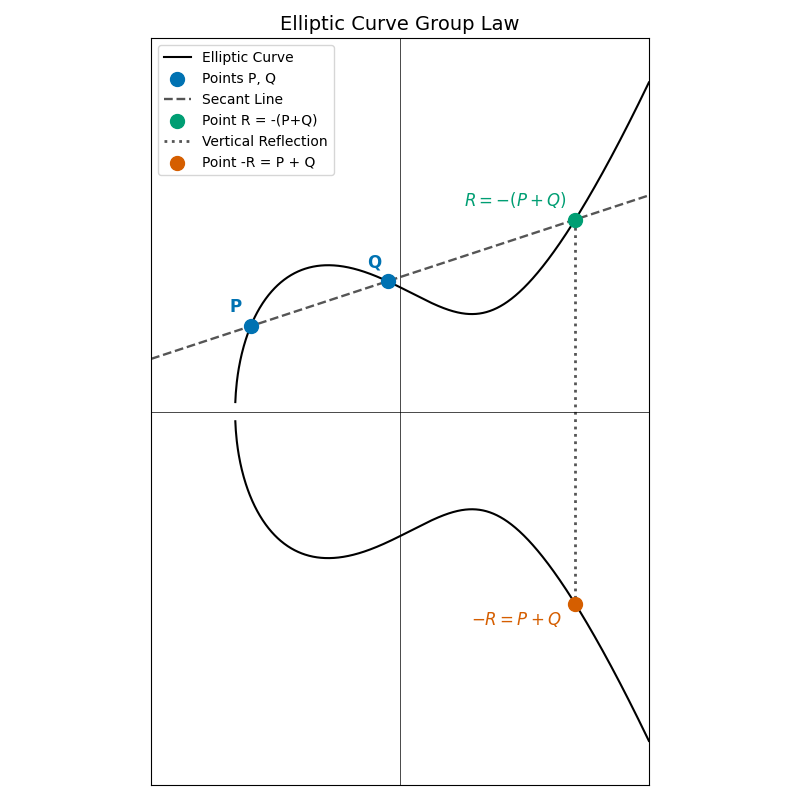
\includegraphics[width=\textwidth]{ecg.png}
\caption{The points $P, Q, R$ are collinear, so their sum is $P + Q + R = O$, where $O$ is the group identity. In particular, $R = -(P+Q)$ and its reflection across the $X$-axis is $-R = P+Q$. \label{fig:grouplaw}}
\end{figure}

In the following, we take B\'{e}zout's theorem for granted (for more details, see Theorem I.7.8 in \cite{Hartshorne}).
\begin{thm}[{B}{\'{e}}zout's {T}heorem]
Let $\F_1$, $\F_2$ be distinct curves in $\P^2(\overline{K})$, having 
degrees $n_1, n_2$, respectively. Let $\F_1 \cap \F_2 = \left\{P_1, \ldots, P_s\right\}$, and say, for each $1 \leq i \leq s$, that point $P_i$ has multiplicity $m_i$. Then $\sum_{i=1}^{s} m_i = n_1n_2$. 
\end{thm}

If $\F_1 = \E$ and $\F_2$ is a line $\ell$, then $\sum_i m_i = 3$. The partitions of $3$ in $\N$ are $1 + 1 + 1$, $1 + 2$, and $3$, so every line intersects $\E$ at $3$ points, counting multiplicities. To fully work out the group structure requires identities, inverses, and the group operation as defined for arbitrary pairs.


First, the point at infinity in projective space $O=(0:1:0) \in \P^2(K)$ is distinguished as the group identity\footnote{See \cite{Silverman} and \cite{Hartshorne} for details, general constructions, and more.}. Next, we find the additive inverse of a non-identity $P \in \G$, i.e.\ we seek $Q \in \G$ such that $P + Q + O = O$. Then  $P = -Q$. By Bezout's theorem, we need a line interpolating $P, Q, O$, and the multiplicities of these points sum to $3$. So we have three cases.

If $P$ has multiplicity $3$, then $P = Q = O$, a contradiction. If $P$ has multiplicity $2$, then $P = Q$ yet $P + Q + O = P + P = 2P = O$.  If $4\alpha^3 + 27\beta^2 \neq 0$, then $\E$ is not singular, a contradiction. So $P$, $Q$, and $O$ form a $3$-set of intersection points, and each has multiplicity $1$. It is easy to check that a  line in $\P^2(\overline{K})$ intersects $\E$ at $O$ if and only if the line is vertical. Thus, to invert $P$, we just reflect $P=(x_P,y_P) \in \P^2$ across the $X$-axis, setting $-P = (x_P, -y_P)$.

This establishes the group identity and inverse elements. It remains to establish the group operation on arbitrary pairs of points, $P$, $Q$. We can assume $P \neq -Q$ as we handled that case already. Given these, to compute $R$ such that $P + Q + R = O$, we find a line $\ell$ interpolating $P$ and $Q$ and consider B\'{e}zout's theorem: the line and $\E$ may intersect at $P$ with multiplicity $3$, $2$, or $1$.

In the first case, $\ell$ intersects $\E$ at $P$ with multiplicity $3$. In this case, $P + P + P = O$ implies $3P = O$, so $P$ is $3$-torsion, implying $\E$ is singular. If $4\alpha^3 + 27\beta^2 \neq 0$, then $\E$ is not singular, a contradiction. 

In the second case, $\ell$ intersects $\E$ at $P$ with multiplicity $2$. In this case $P + P + Q = O$, and so the line interpolating $P$ and $Q$ is tangent to $\E$ at $P$, with multiplicity $2$. That is to say, the second case occurs when we add a point $P$ to itself, ``doubling'' it, computing $P + P = 2P = -Q$. 

In the final case, the line $\ell$ intersects $\E$ at three distinct points $P$, $Q$, and $R$, necessarily with multiplicity $1$ each by B\'{e}zout's theorem. That is to say, the line $\ell$ intersects $\E$ transversally at $P$, $Q$, $R$. For these points, $P + Q + R = O$, so $R = -(P+Q)$. Moreover, we can write the coordinates $R=(x_R, y_R)$ with $y_R = \lambda x_R + \mu$ where $(\lambda, \mu) \in \overline{K}^2$ parameterize the line interpolating $P$ and $Q$.

These rules are sufficient for generating the elliptic curve group $\G(\E)$. In the sequel, we leave $\E$ implicit and denote this $\G$, as we use the same $\E$ throughout. Moreover, the group law as described here is equivalent to a group law defined for rational functions, not merely lines; the proof of this is beyond the scope of this text. See \cite{Silverman} for details.

\subsubsection{Group law and summing points in greater detail}\label{subsec:detail}

We use lines to compute $P + Q$ explicitly as a rational function for a pair $(P, Q) \in (\G \setminus \left\{O\right\})^2$ such that $P \neq \pm Q$; this is useful in our derivations in Appendix \ref{sec:derivation} later. As both are not the identity and $P \neq \pm Q$, the line interpolating $P$ and $Q$ is neither vertical nor tangent to $\E$. By Bezout's theorem, the line must intersect $\E$ transversally at $P$ and $Q$, as well as at a third distinct point $R$, and these intersection points all have multiplicity $1$. 
The group law states $P + Q + R = O$. 
We compute $(x_R, y_R)$ to represent $R$.


Note that, as elements of $\G$, we may write \[P = (x_P:y_P:z_P) = \left\{(x,y,z) \mid \exists \lambda \in K^\times, (x,y,z) = (\lambda x_P,\lambda y_P,\lambda z_P)\right\}\] and $Q = (x_Q:y_Q:z_Q)$ similarly. As non-identity elements, $P \neq O = (0:1:0)$ so $z_P \neq 0$, and the equivalence class $(x_P:y_P:z_P)$ contains a representation of the form $(x,y,1)$ (and similarly for $Q$. Thus, we lose no generality by assuming $z_P=z_Q=1$, in which case we can write $P = (x_P:y_P:1)$ and $Q=(x_Q:y_Q:1)$. Then $P$ and $Q$ may be dehomogenized to affine points $(x_P, y_P)$, $(x_Q, y_Q) \in \E$; we identify $P = (x_P:y_P:1)$ with $(x_P, y_P)$, and similarly for $Q$, in our discussion below, keeping in mind that we are actually transferring between points on the projective plane to points on the affine plane via the dehomogenization and homogenization maps.

Define $\lambda = \frac{y_P - y_Q}{x_P - x_Q}$ and $\mu = y_P - \lambda x_P$ as functions of $P$ and $Q$.
These $\lambda, \mu$ parameterize the interpolating line $\ell(X,Y) = Y - \lambda X - \mu \in K[X,Y]$, and therefore $y_T = \lambda x_T + \mu$ for each $T \in \left\{P, Q, R\right\}$.  Also, since $e(x_T, y_T) = 0$, we have $(\lambda x_T + \mu)^2 = x_T^3 + \alpha x_T + \beta$. Thus, the points $P, Q, R$ have $x$ coordinates which are distinct roots of the third degree polynomial $X^3 - \lambda^2 X^2 + (\alpha - 2\lambda \mu)X + (\beta - \mu^2)$ in $X$.
All the roots are accounted for, so the polynomial splits into linear factors. 
\begin{align}
(X-x_P)(X-x_Q)(X-x_R) &= X^3 - \lambda^2 X^2 + (\alpha - 2\lambda \mu)X + (\beta - \mu^2) 
% X^3 - (x_P + x_Q + x_R)X^2 + (x_Px_Q + x_Px_R + x_Qx_R)X - x_Px_Qx_R
\end{align}
The linear independence of $\left\{1,X,X^2,X^3\right\}$ implies we may match coefficients, so $-\lambda^2 = -x_P - x_Q - x_R$, where $x_P$ and $x_Q$ are already given. Thus we have the following, where we write $x_R$ and $y_R$ as rational functions in the coordinates of $P$ and $Q$:
\begin{align}
x_R &= \lambda^2 - x_P - x_Q \\ 
y_R &= \lambda x_R + \mu
\end{align}
Recalling $\lambda$ and $\mu$ defined above are rational functions, it is clear that these are both rational in $(x_P, x_Q)$, as promised. Thus, the group law demands the following system of equations are satisfied.
\begin{align}
\begin{cases} 
\lambda =& \frac{y_Q-y_P}{x_Q-x_P} \\
\mu =& y_P - \lambda x_P \\
y_P =& \lambda x_P + \mu\\
y_Q =& \lambda x_Q + \mu\\
y_R =& \lambda x_R + \mu\\
y_P^2 =& x_P^3 + \alpha x_P + \beta \\
y_Q^2 =& x_Q^3 + \alpha x_Q + \beta \\
y_R^2 =& x_R^3 + \alpha x_R + \beta 
\end{cases}
\end{align}

\subsubsection{Problems with previous approaches}
This system of $8$ equations with $6$ unknowns influences many computations with derivations in the sequel. Indeed, students of the standard calculus sequence may be familiar with using the \textit{Jacobian} of similar systems of equations to determine if a system is smooth at a point. This yields chain-rule equations when differentiating function field elements at $P$, $Q$, and $R$. 

This is precisely the complication left unaddressed by Eagen in \cite{Eagen}, and tackled by Bassa in \cite{SoundnessForDLP}.  We think the work in \cite{Eagen} intended  characterize solutions to this system as dependent upon $\lambda$ and $\mu$, the only free variables, exactly determining solutions to this system. Had this been correct, the resulting verification equations would have reduced Eagen's claims. This would simplify verification by allowing the chain rule to be computed with respect to the line $Y - \lambda X - \mu = 0$.

While solutions for this system of equations in terms of $\lambda$ and $\mu$ are easily obtainable using Cardano's formula, the solutions are not guaranteed to be rational functions in $\lambda$ and $\mu$. In fact, generally these solutions are not rational, which complicates the application of derivatives beyond the computations in \cite{Eagen}.

On the other hand, by picking $P$ and $Q$, we obtain $x_P, y_P, x_Q, y_Q$, instead over-determining the solution to this system; as Bassa noted, $P = (x_P, y_P)$ and $Q = (x_Q, y_Q)$ form a pair on the surface $(P, Q) \in \E^2$. With this, solutions are rational in $x_P, y_P, x_Q, y_Q$.
However, the $y$ coordinates are \textit{almost} uniquely determined by their corresponding $x$ coordinate. Indeed, for each $T \in \left\{P, Q, R\right\}$, only two elements of $K$ satisfy $y_T^2 = x_T^3 + \alpha x_T + \beta$. Distinguishing which $y_T$ corresponds to the point $T$ simply requires a convention for interpreting a parity/sign bit.
Thus, representing $(x_T,y_T)$ requires only one more bit than representing $x_T$ alone. Thus, we really have five unknown field elements ($x_P, x_Q, x_R, \lambda, \mu$) and $3$ sign bits (one each to uniquely determine $y_P, y_Q, y_R$). Above, we pick $P$ and $Q$, i.e.\ two field elements and two bits, and this is sufficient to uniquely determine $R$, $\lambda$, and $\mu$. 
By over-determining our solutions, we risk that with small probability a solution may not exist, however we only slightly over-determine our solutions by $2$ bits.
For this price, we then obtain rational solutions. 


% This system of equations is important in applying derivations to function field elements, and is not to be overlooked.
% There may be other methods available with different algebraic costs which work over the general case, these constraints are only problematic with negligible probability when $P$ and $Q$ are independently sampled uniformly at random from $\G$. 


\subsection{Divisors over \protect{$\E$}}

For each $T = (x\!:\!y\!:\!z) \in \G$, let $\left[T\right]$ be a formal symbol corresponding to $T$. A \textit{divisor} is a finite sum of these formal symbols. These sums can be summed, so divisors generate an additive group $\text{Div}_K(\E)$. To each $\nu: \E \to \Z$ with finite support, we   assign a unique divisor $[\nu] = \sum_{T \in \E} \nu(T) \left[T\right]$. The \textit{degree} of $\left[\nu\right]$ is $\text{deg}(\left[\nu\right])=\sum_T \nu(T)$. 
Let $\text{Div}_{K}^0(\E)$ denote the set of degree-zero divisors. Note $\text{Div}_{K}^0(\E) \subseteq \text{Div}_K(\E)$ and is closed under addition, i.e.\ is a subgroup.

Given any $f \in K(\E)^\times$, we can define a map $\E \to \Z$  by mapping $T \mapsto \text{ord}_T(f)$, and this has with finite support as the numerator and denominator of $f$ both have finite degree (and hence a $f$ has a finite number of roots and poles, even counting multiplicity). Denote $\text{div}(f) = \sum_{T \in \E} \text{ord}_T(f)[T]$. We say these divisors are \textit{principal divisors} because they are related to computing fractional ideals. Define $\text{Prin}(\E) = \left\{\text{div}(f) \mid f \in K(\E)\right\}$. Note we have the following chain of subgroups: $\text{Prin}(\E) \subseteq \text{Div}_K^0(\E) \subseteq \text{Div}_K(\E)$. In the sequel, define the following relation.
\begin{align}
\R_{\text{div}} =& \left\{(f, [\nu]) \mid f \in K(\E), [\nu] \in \text{Div}_K^0(\E),  \text{ and } \text{div}(f) = [\nu]\right\} \label{theRelation}
\end{align}


We take the following for granted.
\begin{theorem}
Let $f \in K(\E)$, $v_a(f) \setminus \left\{O\right\} = \left\{P_1, \ldots, P_n\right\}$, and $v_a(f^{-1}) \setminus \left\{O\right\} = \left\{Q_1, \ldots, Q_s\right\}$ with $n + s \geq 1$. If each $P_i$ has multiplicity $m_i  \in \N$ and each $Q_j$ has multiplicity $t_j \in \N$, and $\sum_i m_i - \sum_j t_j \neq 0$, then:
\begin{enumerate}[(a)]
\item $\sum_i m_i - \sum_j t_j > 0$ implies $f$ has a pole at $O$ with multiplicity $\sum_i m_i - \sum_j t_j$, 
\item $\sum_i m_i - \sum_j t_j < 0$ implies $f$ has a root at $O$ with multiplicity $\sum_j t_j - \sum_i m_i$, and
\item $\sum_i m_i P_i - \sum_j t_j Q_j = O$.
\end{enumerate}
In particular, $\text{div}(f) = \sum_i m_i [P_i] - \sum_j t_j [Q_j] - (\sum_i m_i - \sum_j t_j)[O]$, $\text{deg}(\text{div}(f)) = 0$, and $\text{div}(f)$ represents a nontrivial decomposition of $O \in \G$, namely $\sum_i m_i P_i - \sum_i t_j Q_j = O$.
\end{theorem}

% Principal divisors admit an abelian group structure and form a subgroup $\texttt{Prin}_K(\E) \subseteq \text{Div}_K^0(\E)$. 

If $f_1, f_2 \in \ff$ have $(v_p(f_1^*) \cup v_p(1/f_1^*)) \cap (v_p(f_2^*) \cup v_p(1/f_2^*)) = \emptyset$, we say $f_1$ and $f_2$ have \textit{disjoint roots and poles}. If $f_1$ and $f_2$ have disjoint roots and poles, it is easy to check that $v_p(f_1^*f_2^*) = v_p(f_1^*)\cup v_p(f_2^*)$ and $v_p(1/(f_1^* f_2^*)) = v_p(1/f_1^*)\cup v_p(1/f_2^*)$. Thus, for such an $f_1, f_2$ pair, we have that $\text{div}(f_1f_2) = \text{div}(f_1)+\text{div}(f_2)$. More generally, $\text{div}$ is a group homomorphism from the multiplicative subgroup of the function field to the additive subgroup $\text{Prin}(\E)$.

Note that if $f_1$ and $f_2$ do not have disjoint roots and poles, then the common roots and poles may partially or completely cancel in the product $f_1f_2$. This expresses itself as terms canceling in the sum $\text{div}(f_1) + \text{div}(f_2)$.



\subsection{Weil's reciprocity}

Every $f \in \overline{K}(\E)$ induces a map on divisors. Indeed, let $\sum_T \eta(T)[T]$ be any divisor, which we denote with $[\eta]$, such that the support of $\eta$ is disjoint from the roots and poles of $f$. Then let $\widehat{f}([\eta]) = \prod_T f(T)^{\eta(T)}$; this is well-defined because the points of $[\eta]$ are disjoint from the roots and poles of $f$.

\begin{theorem}[Weil's Reciprocity Law]
Let $f, g \in \overline{K}(\E)$, with $\text{div}(f) = \sum\limits_T \nu(T) [T]$ and $\text{div}(g) = \sum_T \eta(T) [T]$. Then $\prod\limits_{T \in \G} f(T)^{\eta(T)} = \prod\limits_{S \in \G} g(S)^{\nu(S)}$. 
\end{theorem}

In particular, if $g$ has a degree $1$ polynomial representing its numerator $aX + bY + c + (e)$ and a non-zero constant representing its denominator, say $g = \frac{aX+bY+c}{d}$ for some constants $(a, b, c, d) \in K^4$, then we can re-scale $g$ so that the denominator is $1 + (e)$, say  $g = \ell = \frac{\frac{a}{d}X + \frac{b}{d}Y + \frac{c}{d} + (e)}{1 + (e)}$ without losing any generality; for these, we abuse notation and write $g = \ell = \frac{a}{d} X + \frac{b}{d} Y + \frac{c}{d}$. Then $\widehat{g}(\nu) = \prod_T (ax_T + by_T + c)^{\nu(T)}$.



\subsection{Derivations}

Polynomials admit formal derivatives and partial derivatives as usual: if $f = \sum_i a_i X^i$, define $f^\prime = \sum_i i a_i X^{i-1}$, and if $f = \sum_{i,j} a_{i,j}X^i Y^j$, define $\dX f = \sum_{i,j} ia_{i,j}X^{i-1} Y^j$ and $\dY f = \sum_{i,j} ja_{i,j}X^iY^{j-1}$.

More generally, given any field extension $K \subseteq L$, an additive group homomorphism $d: L \to L$ is said to be a \textit{derivation over} $K$ if $d(K) = \left\{0\right\}$ and $d$ satisfies Leibniz' rule: $d(ab) = d(a)b + ad(b)$. Given an intermediate field, $K \subseteq F \subseteq L$, such that $d(F) \subseteq F$, the restriction of $d$ over $K$ on $L$ to $F$ yields a derivation over $K$ on $F$.  In the case $L=\overline{K}(X,Y)$, derivations $\dX$ and $\dY$ are defined as usual (and $\dZ$ is defined over $\overline{K}(X,Y,Z)$ similarly).
All derivations are linear combinations of these derivations $\dX$, $\dY$, and $\dZ$. Indeed, 
\begin{itemize}
    \item[(i)] for any $a, b \in L$, every linear combination $a(X,Y) \dX + b(X,Y) \dY$ is a derivation over $K$ on $L$, and 
    \item[(ii)] every derivation over $K$ on $L$ is of the form $a(X,Y) \dX + b(X,Y) \dY$, for some $a, b \in \overline{K}(X,Y)$. 
\end{itemize}
For $F \subseteq \overline{K}(X,Y)$, the  derivations satisfying $d(F) \subseteq F$ are precisely the derivations with corresponding $(a, b) \in F^2$.

Similarly, $\overline{K}(X,Y,Z)$ has derivations of the form $d=a\dX + b\dY + c\dZ$ for some $a, b, c \in \overline{K}(X,Y,Z)$, and if all $a, b, c$ are in an intermediate field $K \subseteq F \subseteq \overline{K}(X,Y,Z)$, then $d$ is a derivation on $F$.

Given any derivation $d:L \to L$ over $K$, there is a natural map $\delta:L \to L$ mapping $f \mapsto \frac{df}{f}$. Note that given any $f, g \in L$, we have that 
$$ \delta(fg) = \frac{d(fg)}{fg} = \frac{d(f)g + fd(g)}{fg} = \frac{d(f)}{f} + \frac{d(g)}{g} = \delta(f) + \delta(g).$$
In particular, $\delta$ is a group homomorphism from the multiplicative subgroup of $L$ to the additive group of $L$.


\subsection{Schwarz-Zippel}

We take the following for granted.

\begin{lemm}
Let $0 \neq f \in \overline{K}[Z_1, Z_2, \ldots, Z_n]$ with $\text{deg}(f) = d$, and let $S$ be a finite subset of $\overline{K}$. If $s_1, s_2, \ldots, s_n$ are sampled independently and uniformly from $S$, then the probability that $f(s_1, \ldots, s_n)=0$ is at most $\frac{d}{\left|S\right|}$.
\end{lemm}



\section{Method}

Suppose that a prover and verifier wish to implement a proving scheme in an elliptic curve group setting. In most cases, verification requires satisfying one or more linear constraints coming from the group law of $\G$. That is to say, a proof includes some non-identity group elements $P_1, \ldots, P_n \in \G \setminus \left\{O\right\}$ and integer weights $m_1, \ldots, m_n \in \Z$, then the verification procedure requires checking the $\sum_{i=1}^{n} m_i P_i = O$.

The prover and verifier recall that every principal divisor $\sum_{i=1}^{n} m_i [P_i] - (\sum_{i=1}^{n} m_i)[O]$ corresponds to a decomposition of $O$, so they can merely check whether some divisor  is principal.
The map \textit{div} is a surjective group homomorphism. Therefore, there exists an element $f \in K(\E)$ such that $\text{div}(f) = \sum_i m_i [P_i] - \left(\sum_i m_i\right)[O]$, which can be used as a witness of principality.

% In particular, every $P_i$ with $m_i > 0$ is a root of $f$ with multiplicity $m_i$, and every $P_i$ with $m_i < 0$ is a pole of $f$ with multiplicity $-m_i = \left|m_i\right|$. 

The prover and verifier also recall Weil's reciprocity provides $\widehat{f}(\text{div}(g)) = \widehat{g}(\text{div}(f))$ for every pair $f, g \in K(\E) \subseteq \overline{K}(\E)$. For a fixed $f$, Weil's reciprocity implies an equality of rational functions in the coefficients of $g$ and the coordinates of the points of $\text{div}(g)$; clearing denominators, we obtain a polynomial expression. Evaluating this polynomial at a given $(g, \text{div}(g))$ always yields equality. 

Thus, if $f \in K(\E)$ and some random $(g, \text{div}(g))$ is a root of the polynomial obtained by rationalizing $\widehat{f}(\text{div}(g)) - \widehat{g}(\text{div}(f))$, then the Schwarz-Zippel Lemma implies that the polynomial is the zero polynomial exactly, except with a probability inversely proportional to the cardinality of the set from which we sample $g$.

Hence, checking whether $\widehat{f}(\text{div}(g)) = \widehat{g}([\nu])$ for a random $g$ is sufficient to determine if $\text{div}(f) = [\nu]$, except perhaps with a probability given by the Schwarz-Zippel Lemma. Thus, the prover and verifier can conclude that $\sum_{T \in \G} \nu(T) T = O$, except with that probability. 

To make the checks as efficient as possible, we sample $g$ with degree $1$, and we perform computations under logarithmic derivatives, drastically reducing computational costs.


\subsection{Description}


Let $H:\left\{0,1\right\}^* \to (\G\setminus\left\{O\right\})^2$ be a cryptographic hash function. Define the tuple of algorithms $\Pi = (\texttt{Setup}, \texttt{Prove}, \texttt{Verify})$ as follows. 
\begin{itemize}
\item $\texttt{Setup}(\lambda) \to \texttt{params}$. Input security parameter and output setup parameters $\texttt{params}$.
\item $\texttt{Prove}(\texttt{params}, [\nu]) \to \pi$. The prover does the following:
\begin{enumerate}
\item Compute $\texttt{out} \leftarrow \texttt{MakeWitness}(\texttt{params}, [\nu])$ with Algorithm \ref{alg:makewitness}; if $\texttt{out} = \bot$, output $\bot$ and terminate.
\item Compute $(P, Q) \leftarrow H(\texttt{params}, f, [\nu])$. If $P = \pm Q$, output $\bot$ and terminate.
\item Compute $R = -(P + Q)$. If $P = \pm R$ or $Q = \pm R$ or $\left\{P, Q, R\right\} \cap \left\{P_i\right\}_{i=1}^{n} \neq \emptyset$, output $\bot$ and terminate. %any of the follwoing conditions are satisfied, output $\bot$ and terminate. 
\item Parse the following, if possible; otherwise, output $\bot$ and terminate.
\begin{itemize}
\item $f \leftarrow \texttt{out}$,
\item $\frac{f_1(X) + Yf_2(X) + (e)}{f_3(X) + (e)} \leftarrow f$,
\item $\sum_{i=1}^{n} m_i [P_i] \leftarrow [\nu]$,
\item $(x_P, y_P) \leftarrow P$,
\item $(x_Q, y_Q) \leftarrow Q$, and
\item $(x_R, y_R) \leftarrow R$.
\end{itemize}
\item If $y_T = 0$ for any $T \in \left\{P,Q,R\right\}$, output $\bot$ and terminate.
\item Compute $y_T^\prime = \frac{3x_T^2+\alpha}{2y_T}$ for each $T \in \left\{P, Q, R\right\}$.
\item If $y_T^\prime = \lambda$  or $f(T) = 0$ or $f_3(x_T) = 0$ for any $T \in \left\{P, Q, R\right\}$, output $\bot$ and terminate.


\item \label{repeatstep} Compute the following:
\begin{align}
\Delta X =& x_Q - x_P\\
\Delta Y =& y_Q - y_P\\
\lambda =& \frac{\Delta Y}{\Delta X} \\
\mu =& y_P - \lambda x_P \\
f_X =& \frac{(f_1^\prime + Yf_2^\prime)f_3 - f\cdot f_3^\prime + (e)}{f_3^2 + (e)}\\
f_Y =& \frac{f_2 + (e)}{f_3 + (e)}
\end{align}

\item Compute the following:
\begin{align}
A_i =& (y_i - \lambda x_i - \mu)^{-1}\text{ for each }1 \leq i \leq n \\
B_1 =& \frac{2y_Pf_X(P) + (3x_P^2+\alpha) f_Y(P)}{2y_Pf(P)(3x_P^2+\alpha - 2\lambda y_P)} \\
B_2 =& - \frac{2\lambda y_P(2y_Rf_X(R) + (3x_R^2+\alpha) f_Y(R))(3x_P^2+\alpha - 2y_P(\lambda + \Delta X))}{2y_Py_Rf(R)(3x_P^2+\alpha-2y_P \lambda )\Delta X} \\
B_3 =& \frac{2y_Qf_X(Q) + (3x_Q^2+\alpha) f_Y(Q)}{2y_Qf(Q)(3x_Q^2+\alpha - 2\lambda y_Q)} \\
B_4 =& \frac{2\lambda y_Q(2y_Rf_X(R) + (3x_R^2+\alpha)f_Y(R))(3x_Q^2+\alpha - 2y_Q(\lambda + \Delta X))}{2y_Qy_Rf(R)(3x_Q^2+\alpha  - 2\lambda y_Q) \Delta X}
\end{align}


\item Output $\pi = (f,  A_1, \ldots, A_n, B_1, B_2, B_3, B_4)$. 
\end{enumerate}


\item $\texttt{Verify}(\texttt{params}, [\nu], \pi) \to b \in \zo$.
\begin{enumerate}
\item Parse $\sum_{i=1}^n m_i P_i \leftarrow [\nu]$ and  $(f,  A_1, \ldots, A_n, B_1, B_2, B_3, B_4) \leftarrow \pi$, and $\frac{f_1(X) + Yf_2(X) + (e)}{f_3(X) + (e)} \leftarrow f$  if possible; if not, output $0$ and terminate.
\item Compute challenge points $(P, Q) \leftarrow H(\texttt{params}, f, [\nu])$. If $P = \pm Q$, output $0$ and terminate.
\item Compute $R = -(P + Q)$. If $P = \pm R$ or $Q = \pm R$ or $\left\{P, Q, R\right\} \cap \left\{P_i\right\}_{i=1}^{n} \neq \emptyset$, output $\bot$ and terminate. %any of the follwoing conditions are satisfied, output $\bot$ and terminate.
\item Carry out step \ref{repeatstep} from \texttt{Prove}.
\item Compute the following.
\begin{align}
% \Delta X =& x_Q - x_P \\
% \Delta Y =& y_Q - y_P \\
% \lambda =& \frac{\Delta Y}{\Delta X} \\
% \mu =& y_P - \lambda x_P \\
% R =& -(P + Q) \\
b_1 =& 2y_Pf(P)(3x_P^2+\alpha-2\lambda y_P) \\
c_1 =& 2y_Pf_X(P) + (3x_P^2+\alpha) f_Y(P)\\
b_2 =& 2y_Py_Rf(R)(3x_P^2+\alpha-2y_P \lambda ) \Delta X\\
c_2 =& - 2\lambda y_P(2y_Rf_X(R) + (3x_R^2+\alpha) f_Y(R))(3x_P^2+\alpha - 2y_P(\lambda + \Delta X))\\
b_3 =& 2y_Qf(Q)(3x_Q^2+\alpha - 2\lambda y_Q)\\
c_3 =& 2y_Qf_X(Q) + (3x_Q^2+\alpha) f_Y(Q) \\
b_4 =& \left(2y_Qy_Rf(R)(3x_Q^2+\alpha  - 2\lambda y_Q) \Delta X\right)\\
c_4 =& 2\lambda y_Q(2y_Rf_X(R) + (3x_R^2+\alpha)f_Y(R))(3x_Q^2+\alpha - 2y_Q(\lambda + \Delta X))
\end{align}

\item If any $1 \leq i \leq n$ has $(y_i - \lambda x_i - \mu)A_i \neq 1$, output $0$ and terminate.

\item If any $1 \leq i \leq 4$ has $b_iB_i \neq c_i$, output $0$ and terminate.

\item If $B_1 + B_2 + B_3 + B_4 \neq \sum_i m_i A_i$, output $0$ and terminate.

\item Otherwise, output $1$ and terminate.

\end{enumerate}

\end{itemize}

\begin{table}[H]
    \centering
    \begin{tabular}{|l|}
    \hline
    $\texttt{MakeWitness}([P_i]) \to \texttt{out} \in \{\bot\} \cup K(\E)$ \\
    \hline
    If no points were provided, output $\bot$ and terminate. \\
    If the input points do not sum to the identity $O$, or any input point is $O$, \\
    \quad output $\bot$ and terminate. \\
    Initialize an empty queue $\texttt{queue} = \emptyset$. \\
    Parse the point set into pairs. For each pair $(P_{2j},P_{2j+1})$: \\
    \quad (If the number of points is odd, set $P_{2j+1} \leftarrow O$ for the final pair.) \\
    \quad Compute: \\
    \quad\quad $T_j = P_{2j} + P_{2j+1} \in \E$,\\
    \quad\quad $\ell_j$, the interpolation line divisor: $\ell_j = \texttt{line}(P_{2j},P_{2j+1}) \in K(\E)$ \\
    \quad Queue $(2, T_j, \ell_j)$ into $\texttt{queue}$. \\
    % Set $e(X,Y) \leftarrow  Y^2 - X^3 - aX - b$, the curve modulus. \\
    While $\texttt{len}(\texttt{queue}) > 1$: \\
    \quad Initialize empty queue $\texttt{nextQueue} = \emptyset$. \\
    \quad If $\texttt{len}(\texttt{queue}) \equiv 1 \mod 2$: \\
    \quad\quad Pop the last element from $\texttt{queue}$ and push it onto $\texttt{nextQueue}$. \\
    \quad Let $N = \lfloor\texttt{len}(\texttt{queue})/2\rfloor$. \\
    \quad For $1 \leq j \leq N$: \\
    \quad\quad Pop $(m_a, T_a, f_a)$ and $(m_b, T_b, f_b)$ from $\texttt{queue}$. \\
    \quad\quad Compute: \\
    \quad\quad\quad $T_{j} = T_{a} + T_{b}$,\\
    \quad\quad\quad $\widehat{\ell}_j = \texttt{line}(T_{a}, T_{b})$,\\
    \quad\quad\quad $\text{numerator} = f_{a} \cdot f_{b} \cdot \widehat{\ell}_j \mod e(X,Y)$,\\
    \quad\quad\quad $\text{denominator} = \texttt{line}(T_{a}, -T_{a}) \cdot \texttt{line}(T_{b}, -T_{b})$,\\
    \quad\quad Set $g := \text{numerator}/\text{denominator}$.\\
    % \quad\quad Truncate zero-coefficient terms from $q$ based on total merged points.\\
    \quad\quad Queue $(m_a+m_b, T_{j}, g)$ into $\texttt{nextQueue}$. \\
    \quad Set $\texttt{queue} \leftarrow \texttt{nextQueue}$. \\
    Pop $(m, T, f) \leftarrow \texttt{queue}$. \\
    % Truncate zero-coefficient terms from $f$ based on total number of input points. \\
    If $T \neq O$, output $\bot$ and terminate. \\
    Output $f$. \\
    \hline
    \end{tabular}    
    \caption{Constructing a rational function whose divisor interpolates a list of elliptic curve points.}
    \label{alg:makewitness}
\end{table}


% \begin{table}[H]
%     \centering
%     \begin{tabular}{|l|}
%     \hline
%     $\texttt{MakeWitness}(\texttt{params}, [\nu]) \to \texttt{out} \in \left\{\bot\right\} \cup K(\E)$ \\
%     \hline
%     Parse $\sum_{i=1}^{n} m_i P_i \leftarrow [\nu]$. \\
%     Compute $\texttt{out} \leftarrow \texttt{MakePairs}(\texttt{params}, [\nu])$. \\
%     If $\texttt{out} = \bot$, output $\bot$ and terminate. \\
%     Otherwise, parse $\left\{\texttt{pair}_j\right\}_{j=1}^M \leftarrow \texttt{out}$. \\
%     Initialize empty $\texttt{queue} = \emptyset$. \\
%     For each $1 \leq j \leq M$: \\
%     \quad Parse $(Q_{j,1},Q_{j,2}) \leftarrow \texttt{pair}_j$. \\
%     \quad Parse $(x_{j,1}, y_{j,1}) \leftarrow Q_{j,1}$ and $(x_{j,2}, y_{j,2}) \leftarrow Q_{j,2}$. \\
%      \quad Compute: 
%      \quad \quad $\ell_j = (X-x_{j,1})(y_{j,2}-y_{j,1})+(x_{j,2}-x_{j,1})(Y-y_{j,1})$ \\
%      \quad \quad $T_j = Q_{j,1} + Q_{j,2} \in \G$ \\
%     % \quad Set $\texttt{group\_law}_j = (Q_{j,1},Q_{j,2},T_j)$. \\
%     \quad  Queue $(T_j, \ell_j)$ into $\texttt{queue}$. \\
%     % \quad Set $\texttt{result} = 1 \in K$. \\
%      While $\texttt{len}(\texttt{queue}) > 1$: \\
%     \quad If $\texttt{len}(\texttt{queue}) \equiv 1 \ (\text{mod }2)$, set $\texttt{reserved} \leftarrow \texttt{queue}[-1]$ \\
%     \quad Let $N = \texttt{len}(\texttt{queue})/2$. \\
%     \quad For $1 \leq j \leq N$: \\
%     \quad \quad Pop $(T_{2j}, f_{2j}) \leftarrow \texttt{queue}$ and $(T_{2j+1}, f_{2j+1}) \leftarrow \texttt{queue}$. \\
%     % \quad Pop each pair $(\texttt{group\_law}_j, f_{j_1}), (T_{j_2}, f_{j_2}) \leftarrow \texttt{unprocessed}$: \\
%     \quad \quad Parse: \\
%     % \quad \quad \quad $(Q_{2j,1}, Q_{2j,2}, T_{2j}) \leftarrow \texttt{group\_law}_{2j}$ \\
%     % \quad \quad \quad $(Q_{2j+1,1}, Q_{2j+1,2}, T_{2j+1}) \leftarrow \texttt{group\_law}_{2j+1}$ \\
%     \quad \quad\quad $(x_{2j},y_{2j}) \leftarrow T_{2j}$ and $(x_{2j+1},y_{2j+1}) \leftarrow T_{2j+1}$. \\
%     \quad\quad Compute: \\
%     \quad\quad\quad $S_j = T_{2j}+T_{2j+1}$ \\
%     \quad\quad\quad$\widetilde{f}_j = f_{2j}\cdot f_{2j+1}$\\
%     \quad\quad \quad $\widehat{\ell}_j = (X-x_{2j})(y_{2j+1}-y_{2j})+(x_{2j+1}-x_{2j})(Y-y_{2j})$. \\
%     \quad\quad\quad $g_{2j} = X-x_{2j}$, $g_{2j+1}=X-x_{2j+1}$. \\
%     \quad\quad \quad $\widetilde{f}_j \leftarrow  \cdot \frac{\widetilde{f}_j\widehat{\ell}_j}{g_{2j}g_{2j+1}}$. \\
%     % \quad\quad\quad Set $\texttt{result} \leftarrow \texttt{result} \cdot \rho \cdot (X-x_{j_1})^{-1}(X-x_{j_2})^{-1}$. \\
%     \quad\quad Queue $(S_j, \widetilde{f}_j)$ into $\texttt{queue}$. \\
%     \quad Queue $\texttt{reserved}$ into $\texttt{queue}$. \\
%     Pop $(T, f) \leftarrow \texttt{queue}$. \\
%     If $T \neq O$, output $\bot$ and terminate. \\
%     Otherwise, return $f$. \\
%     \hline
%     \end{tabular}    
%     \caption{Constructing a rational function whose divisor interpolates a set of elliptic curve points.}
%     \label{alg:makewitness}
% \end{table}


% \begin{table}[H]
%     \centering
%     \begin{tabular}{|l|}
%     \hline
%     $\texttt{MakePairs}(\texttt{params}, [\nu]) \to \left\{\bot, \left\{\texttt{pairs}_j\right\}_{j=1}^M\right\}$ \\
%     \hline
%     Parse $\sum_{i=1}^{n} m_i P_i \leftarrow [\nu]$. \\
%     If $n = 0$ or any $P_i = \mathcal{O}$ or $\sum_i P_i \ne \mathcal{O}$, output failure symbol $\bot$ and terminate. \\
%     Set $\texttt{points} = (\underbrace{P_1, \ldots, P_1}_{m_1\text{ times}}, \underbrace{P_2, \ldots, P_2}_{m_2\text{ times}}, P_3, \ldots, P_{n-1}, \underbrace{P_n, P_n, \ldots, P_n}_{m_n\text{ times}})$. \\
%     If $\texttt{len}(\texttt{points}) \equiv 1 \, (\text{mod }2)$: \\
%     \quad Compute $-P_n$ \\
%     \quad Append $-P_n$ to $\texttt{points}$, i.e.\\
%     \quad\quad $\texttt{points} = (\underbrace{P_1, \ldots, P_1}_{m_1\text{ times}}, \underbrace{P_2, \ldots, P_2}_{m_2\text{ times}}, P_3, \ldots, P_{n-1}, \underbrace{P_n, P_n, \ldots, P_n}_{m_n\text{ times}}, -P_n)$. \\
%     Let $M = \texttt{len}(\texttt{points})/2$. \\
%     For each $1 \leq j \leq M$, set $\texttt{pair}_j = (\texttt{points}_{2j}, \texttt{points}_{2j+1})$. \\
%     Return $\left\{\texttt{pairs}_j\right\}_{j=1}^{M}$. \\
%     \hline
%     \end{tabular}    
%     \caption{Partition a divisor (with no identity points and which sums to $O$) into pairs of points and possibly an additional reserved point.}
%     \label{alg:makepairs}
% \end{table}

The runtime of $\texttt{MakeWitness}$ is $O(n^2)$.


Usage of this scheme is somewhat self-evident; for example, to prove that a scalar multiplication has been performed correctly, say $P = aG$ for some $G \in \G \setminus\left\{O\right\}$ and some $1 \leq a < \text{ord}(\G)$, the prover runs $\texttt{MakeWitness}$ with $[\nu] = a[G] + [-P]$.

\subsection{Security properties}\label{sec:SecurityProps}

It should be clear that, if $[\nu]$ is a nontrivial decomposition of $O$ into a sum of non-identity points, then $\texttt{MakePairs}$ certainly does not output $\bot$. 

\begin{lemm}
\label{lem:number_collinear_triples}
Let $\left\{P_1, \ldots, P_n\right\}$ be a subset of $\G$. Let $\texttt{Collinear}(\G)$ be the set of $3$-sets of points, say $\left\{P, Q, R\right\} \subseteq \G$, which are distinct, on $\E$, and collinear.
Then $\mathbb{P}\left[\texttt{Collinear} \cap \left\{P_1, \ldots, P_n\right\} \neq \emptyset\right] = \frac{1}{6}\left(\left|\G\right|-1\right)\left(\left|\G\right|-2\right)$.
\end{lemm}
\begin{proof}
There are $\left|\G\right| - n$ choices of $P$ which do not collide with any $P_i$. After selecting $P$, there are $\left|\G\right| - (n+1)$ choices of $Q$ which do not collide with any $P_i$. 
\end{proof}

We also have the following.

\begin{lemm}
\label{lem:witnessCorrectness}
If $[\nu]$ is a nontrivial decomposition of $O$ into a sum of non-identity points, then $\texttt{MakeWitness}$ runs in time $t = O()$, succeeds with certainty, and outputs $f$ such that $\text{div}(f) = [\nu] - \text{deg}([\nu])[O]$.
\end{lemm}


We omit the proof for this claim for now; see upcoming work. 

\begin{theorem}\label{thm:DivisorCompleteness}
Let $\G$ have prime order $q > 3$. $\Pi$ is a complete proving system for the relation $\R$ from Equation \ref{theRelation} with the completeness error $\kappa \leq \frac{2n + 8}{\left|\G\right|} \in O(1/\left|\G\right|)$.
\end{theorem}
\begin{proof}
Presume that $f \in K(\E)$, $[\nu] = \text{div}(f)$, and the prover honestly executes $\texttt{Prove}$. Then the following occurs.
\begin{enumerate}[(a)]
\item The prover computes $\texttt{out} \leftarrow \texttt{MakeWitness}(\texttt{params},[\nu])$. Following Lemma \ref{lem:witnessCorrectness}, this algorithm does not fail and $\texttt{out} = f \in K(\E)$, where $f = \frac{f_1(X) + Yf_2(X) + (e(X,Y))}{f_3(X) + (e(X, Y))}$.
\item The prover computes $(P,Q) \leftarrow H(\texttt{params}, f, [\nu])$ and fails if $P = \pm Q$. Under the random oracle model, $H$ has output uniformly sampled from $(\G \setminus \left\{O\right\})^2$. There are $\left|\G\right| - 1$ pairs $(P, P)$ with $P \neq O$. There are $\frac{1}{2}\left(\left|\G\right| - 1\right)$ unordered pairs $(P, -P)$ with $P \neq O$. Since the order of $\G$ is $q$, every non-identity element has order $q > 3$, so no group element $P$ satisfies $P + P = O$. Hence,  we have $\frac{3}{2}\left(\left|\G\right| - 1\right)$ pairs which may cause the prover to output $\bot$, out of $(\left|\G\right|-1)^2$ . In particular, the prover fails with probability $\frac{3}{2\left(\left|\G\right|-1\right)}$.

\item The prover computes $R = -(P+Q)$. Note the constraints that $P, Q \neq O$ and $P \neq \pm Q$ admit an interpolating line $\ell$ which is not vertical and not tangent to $\E$, so $R \neq \pm P$ and $R \neq \pm Q$.

Since $(P, Q)$ are sampled from a random oracle, this line $\ell$ is sampled uniformly from the set of all lines in $K[X,Y]/I(\E/K)$ which are vertical and not tangent to $\E$. Thus, the set $\left\{P,Q,R\right\}$ is sampled uniformly from the set of all $3$-sets of  collinear non-identity points on $\E$. Each such triple is uniquely determined by $P$ and $Q$. By Lemma \ref{lem:number_collinear_triples}, there are $\frac{1}{6}\left(\left|\G\right| - 1\right)\left(\left|\G\right| - 2\right)$ such triples. On the other hand, there are $\left|\G \setminus \left\{O, P_1, \ldots, P_n\right\}\right| = \left|\G\right| - n - 1$ group elements which miss the divisor points, so $\frac{1}{6}\left(\left|\G\right| - n - 1\right)\left(\left|\G\right| - n - 2\right)$ triples do not collide with the points $\left\{P_1, \ldots, P_n\right\}$. Hence, the probability of failure here is $\mathbb{P}\left[\left\{P, Q, R\right\} \cap \left\{P_1, \ldots, P_n\right\} \neq \emptyset\right]  = 1-\left(1-\frac{n}{\left|\G\right|-1}\right)\left(1-\frac{n}{\left|\G\right|-2}\right) = O\left(\frac{n^2}{\left|\G\right|^2}\right)$. This is asymptotically $O(\left|\G\right|^{-2})$, but concrete choices of $n$ and $\G$ may lead to insecurity. 
% See Section \ref{} \free{EMPTY REF????} for more about this.

\item As the prover is honest, parsing in this step succeeds with certainty.

\item 
Unless the prover already failed, we have that $\left\{P, Q, R\right\}$ misses the roots and poles of $f$, so $f(T)$ and $f_3(x_T)$ are both non-zero and well-defined for each $T \in \left\{P,Q,R\right\}$. Also, at most one point on $\E$ has a zero $y$-coordinate. There are $\left|\G\right|-2$ lines $\ell$ which interpolate the point with a zero $y$-coordinate, out of $\frac{1}{6}\left(\left|\G\right|-1\right)\left(\left|\G\right|-2\right)$. Hence, there is a probability of $\frac{6}{\left|\G\right|-1}$ that the prover outputs $\bot$ in this step.

\item As the prover is honest, computations in this step succeed with certainty.

\item If the prover did not fail before this point, then $\left\{P,Q,R\right\} \cap \left\{P_i\right\}_{i=1}^{n} = \emptyset$, where these $P_i$ exhaust the roots and poles of $f$. Hence, $f(P)$, $f(Q)$, $f(R)$, are each non-zero and well-defined, so the prover succeeds in this step with certainty. 

\item If the prover has not failed before this step, then all the computations in this step succeed with certainty.

\item The prover outputs $\pi = (f, A_1, \ldots, A_n, B_1, B_2, B_3, B_4)$.
\end{enumerate}


If the prover does not fail, then during verification the following occurs.
\begin{enumerate}[(a)]
\item Parsing succeeds with certainty here, so the verifier does not output $0$ in this step.
\item Since the prover is honest and did not fail, the witness is a valid function field element, and the verifier obtains $(P, Q)$ with $P \neq \pm Q$ without outputting $0$ here.
\item The verifier computes $R = -(P+Q)$ and checks for a collision. Since the prover is honest and did not fail, the points $P, Q, R$ do not collide with the points $\left\{P_i\right\}$, so the verifier does not output $0$ in this step.

\item If the verifier has not yet terminated, then all the computations in this step succeed with certainty and we obtain the following.
\begin{align}
b_1 =& 2y_Pf(P)(3x_P^2+\alpha-2\lambda y_P) \\
c_1 =& 2y_Pf_X(P) + (3x_P^2+\alpha) f_Y(P)\\
b_2 =& 2y_Py_Rf(R)(3x_P^2+\alpha-2y_P \lambda ) \Delta X\\
c_2 =& - 2\lambda y_P(2y_Rf_X(R) + (3x_R^2+\alpha) f_Y(R))(3x_P^2+\alpha - 2y_P(\lambda + \Delta X))\\
b_3 =& 2y_Qf(Q)(3x_Q^2+\alpha - 2\lambda y_Q)\\
c_3 =& 2y_Qf_X(Q) + (3x_Q^2+\alpha) f_Y(Q) \\
b_4 =& \left(2y_Qy_Rf(R)(3x_Q^2+\alpha  - 2\lambda y_Q) \Delta X\right)\\
c_4 =& 2\lambda y_Q(2y_Rf_X(R) + (3x_R^2+\alpha)f_Y(R))(3x_Q^2+\alpha - 2y_Q(\lambda + \Delta X))
\end{align} 

\item Each $A_i = (y_i - \lambda x_i - \mu)$ since the prover was honest, so $(y_i - \lambda x_i - \mu)A_i = 1$ with certainty, and the verifier does not output $0$ in this step.

\item We have the following, also since the prover was honest.
\begin{align}
B_1 =& \frac{2y_P f_X(P) + (3x_P^2+\alpha)f_Y(P)}{2y_Pf(P)(3x_P^2+\alpha-2\lambda y_P)} = \frac{c_1}{b_1}\\
B_2 =& - \frac{2\lambda y_P(2y_Rf_X(R) + (3x_R^2+\alpha) f_Y(R))(3x_P^2+\alpha - 2y_P(\lambda + \Delta X))}{2y_Py_Rf(R)(3x_P^2+\alpha-2\lambda y_P)\Delta X} = \frac{c_2}{b_2} \\
B_3 =& \frac{2y_Qf_X(Q) + (3x_Q^2+\alpha) f_Y(Q)}{2y_Qf(Q)(3x_Q^2+\alpha - 2\lambda y_Q)} = \frac{c_3}{b_3} \\
B_4 =& \frac{2\lambda y_Q(2y_Rf_X(R) + (3x_R^2+\alpha)f_Y(R))(3x_Q^2+\alpha - 2y_Q(\lambda + \Delta X))}{2y_Qy_Rf(R)(3x_Q^2+\alpha  - 2\lambda y_Q) \Delta X} = \frac{c_4}{b_4}
\end{align}
Thus, each $b_i B_i = c_i$, so the verifier does not output $0$ in this step.

\item In Equation \ref{deltafhat} of the Appendix, we show $\delta(\widehat{f}(X_P,Y_P,X_Q,Y_Q))\mid_{P,Q} = B_1 + B_2 + B_3 + B_4$.   We also have $\widehat{f}(x_P,y_P,x_Q,y_Q) = f(P)f(Q)f(R)$, and by Weil's reciprocity, $f(P)f(Q)f(R) = \prod_{i=1}^{n} (y_i - \lambda x_i - \mu)^{m_i}$, where $Y - \lambda X - \mu$ is the line interpolating $P$, $Q$, and $R$. Hence, $\delta(\widehat{f})\mid_{P,Q} = \sum_{i=1}^{n} \frac{m_i}{y_i-\lambda x_i - \mu}$. The verifier checked above that $(y_i-\lambda x_i - \mu)A_i = 1$, so $\delta(\widehat{f})\mid_{P,Q} = \sum_i m_i A_i$, implying verification is passed.
\end{enumerate}

Let $\rho_b = \frac{3}{2\left|\G\right| - 2}$ be the probability of failure in step $b$. Let $\rho_c = 1 - \left(1-\frac{n}{\left|\G\right|-1}\right)\left(1-\frac{n}{\left|\G\right|-2}\right)$ be the probability of failure in step $c$. Let $\rho_e = \frac{6}{\left|\G\right|-1}$ be the probability of failure in step $e$.
Then, by the law of total probability, the completeness error of the protocol is $\rho_b + (1-\rho_b)(\rho_c + (1-\rho_c)\rho_e)$. This simplifies
% \footnote{We used Mathematica to simplify these; manually checking this is an important improvement in upcoming versions of this paper.} 
as follows: 


% \[\frac{3}{2\left|\G\right|-2} + \left(\frac{2\left|\G\right| - 5}{2\left|\G\right|-2}\right)\Bigg(1 - \left(1-\frac{n}{\left|\G\right|-1}\right)\left(1-\frac{n}{\left|\G\right|-2}\right) + \left(1-\frac{n}{\left|\G\right|-1}\right)\left(1-\frac{n}{\left|\G\right|-2}\right)\left(\frac{6}{\left|\G\right|-1}\right)\Bigg)\]

\begin{align*}
    \kappa &=  \frac{3 (5 \left|\G\right|-11)}{2 (\left|\G\right|-1)^2} + \frac{n(\left|\G\right|-7) (2 \left|\G\right|-5) (2 \left|\G\right|-(n+3))}{2(\left|\G\right|-2) (\left|\G\right|-1)^3} \\
    &\approx  \frac{15 \left|\G\right|}{2 \left|\G\right|^2} + \frac{ 4 n\left|\G\right|^3}{2\left|\G\right|^4} \\
    &= \frac{4n + 15}{2 \left|\G\right|} \\
    & \leq \frac{2n + 8}{\left|\G\right|}
    % &= \frac{4n+15}{\left|\G\right|}\left(1 - \frac{78+44n + 2n^2}{4n+15} \left|\G\right|^{-1} + \frac{129+127n + 19n^2}{4n+15} \left|\G\right|^{-2} - \frac{66+105n + 35n^2}{4n+15} \left|\G\right|^{-3}\right)  \\    
    % &\approx \frac{4n+15}{\left|\G\right|}\left(1 - \frac{n}{2\left|\G\right|}\left(1 - \frac{19}{2\left|\G\right|}\left(1 -  \frac{35}{19\left|\G\right|}\right)\right)\right) \leq \frac{4n+15}{\left|\G\right|}
\end{align*}
\end{proof}





\begin{theorem}\label{thm:DivisorSoundness}
$\Pi$ is a sound proving system for the relation 
$$\R = \left\{(f, \text{div}(f)) \mid f \in K(\E) \text{ and } \text{div}(f) \in Prin(\G) \right\}.$$
\end{theorem}
\begin{proof}
Assume $\texttt{Verify}(\texttt{params}, \sum_{i=1}^{n} m_i [P_i], \pi) = 1$. Then $\pi = (f,  A_1, \ldots, A_n, B_1, B_2, B_3, B_4)$ for some $f \in K(\E)$ and some $A_1, \ldots, A_n, B_1, B_2, B_3, B_4 \in K$, otherwise the verifier would output $0$ in the first step, a contradiction. Moreover, the verifier computes challenge points $(P, Q) \leftarrow H(\texttt{params}, f, \sum_{i=1}^{n} m_i [P_i])$ such that $P \neq \pm Q$, otherwise the verifier would output $0$ in the second step, a contradiction.  The verifier computes $R = -(P + Q)$, and finds that $P \neq \pm R$ and $Q \neq \pm R$ and $\left\{P, Q, R\right\} \cap \left\{P_i\right\}_{i=1}^{n} = \emptyset$, otherwise the verifier would output $0$ in the third step, a contradiction. Thus, the verifier successfully computes $\Delta X$, $\Delta Y$, $\lambda$, $\mu$, $R$, and $(b_i, c_i)$ for $i=1$, $2$, $3$, and $4$, yielding the following 
% \free{ADDRESS THIS FOOTNOTE} \footnote{MACRO THESE}.
\begin{align}
\Delta X =& x_Q - x_P \\
\Delta Y =& y_Q - y_P \\
\lambda =& \frac{\Delta Y}{\Delta X} \\
\mu =& y_P - \lambda x_P \\
b_1 =& 2y_Pf(P)(3x_P^2+\alpha-2\lambda y_P) \\
c_1 =& 2y_Pf_X(P) + (3x_P^2+\alpha) f_Y(P)\\
b_2 =& 2y_Py_Rf(R)(3x_P^2+\alpha-2y_P \lambda ) \Delta X\\
c_2 =& - 2\lambda y_P(2y_Rf_X(R) + (3x_R^2+\alpha) f_Y(R))(3x_P^2+\alpha - 2y_P(\lambda + \Delta X))\\
b_3 =& 2y_Qf(Q)(3x_Q^2+\alpha - 2\lambda y_Q)\\
c_3 =& 2y_Qf_X(Q) + (3x_Q^2+\alpha) f_Y(Q) \\
b_4 =& \left(2y_Qy_Rf(R)(3x_Q^2+\alpha  - 2\lambda y_Q) \Delta X\right)\\
c_4 =& 2\lambda y_Q(2y_Rf_X(R) + (3x_R^2+\alpha)f_Y(R))(3x_Q^2+\alpha - 2y_Q(\lambda + \Delta X))
\end{align}
At this point, the verifier finds $(y_i - \lambda x_i - \mu)A_i = 1$ for each $i=1$, $2$, $\ldots$, $n$, otherwise the verifier would output $0$ after this check. Thus, the verifier is assured each $A_i = (y_i - \lambda x_i - \mu)^{-1}$ with certainty.
Then the verifier finds that $b_iB_i = c_i$ for each $i=1$, $2$, $3$, and $4$, otherwise the verifier would output $0$ after this check. Thus, the verifier is assured that each of these satisfy $B_i = c_i/b_i$ with certainty. Lastly, the verifier finds that $B_1 + B_2 + B_3 + B_4 = \sum_i m_i A_i$. Hence, the verifier is assured that the following is satisfied with certainty.
\[\frac{c_1}{b_1} + \frac{c_2}{b_2} + \frac{c_3}{b_3} + \frac{c_4}{b_4} = \sum_i \frac{m_i}{y_i-\lambda x_i \mu}\]
Moreover, since the verifier computed these $c_i, b_i$ as above, the verifier concludes the following.

\begin{align*}
    & \frac{2y_Pf_X(P) + (3x_P^2+\alpha) f_Y(P)}{2y_Pf(P)(3x_P^2+\alpha-2\lambda y_P)} 
    - \frac{2\lambda y_P(2y_Rf_X(R) + (3x_R^2+\alpha) f_Y(R))(3x_P^2+\alpha - 2y_P(\lambda + \Delta X))}{2y_Py_Rf(R)(3x_P^2+\alpha-2y_P \lambda ) \Delta X} \\
    &+ \frac{2y_Qf_X(Q) + (3x_Q^2+\alpha) f_Y(Q)}{2y_Qf(Q)(3x_Q^2+\alpha - 2\lambda y_Q)} + \frac{2\lambda y_Q(2y_Rf_X(R) + (3x_R^2+\alpha)f_Y(R))(3x_Q^2+\alpha - 2y_Q(\lambda + \Delta X))}{2y_Qy_Rf(R)(3x_Q^2+\alpha  - 2\lambda y_Q) \Delta X} \\
    &= \sum_i \frac{m_i}{y_i-\lambda x_i \mu}
\end{align*}

By Equations \ref{dfp} and \ref{dfq} in the Appendix, the verifier knows the following.

\[\frac{2y_Pf_X(P) + (3x_P^2+\alpha) f_Y(P)}{2y_Pf(P)(3x_P^2+\alpha-2\lambda y_P)} = \delta(f(X,Y))\mid_{(X, Y)=(x_P,y_P)}\]
\[\frac{2y_Qf_X(Q) + (3x_Q^2+\alpha) f_Y(Q)}{2y_Qf(Q)(3x_Q^2+\alpha - 2\lambda y_Q)} = \delta(f(X,Y))\mid_{(X,Y)=(x_Q,y_Q)}\]
Also, the verifier knows the derivation $d$ (and therefore the logarithmic derivative $\delta$) on $K(\E)$ over $K$ extends to the function fields for the product variety $K(\E^2)$. Thus, $\delta(f(X_R, Y_R))\mid_{(P,Q)}$ is as follows due to Equation \ref{dfr}.


% \begin{align}
% df(R) =& f_X(R)dX_R + f_Y(R) dY_R \\
% =& (f_X(R) + Y^\prime_R f_Y(R))dX_R \\
% df(R) =& \frac{2\Lambda(f_X(R) + Y^\prime_R f_Y(R))}{\Delta X}\Big(\left(Y_Q^\prime - \Lambda - \Delta X\right) dX_Q  - \left(Y_P^\prime - \Lambda + \Delta X\right)dX_P\Big) \label{dfr}
% \end{align}

\begin{align}
% \frac{2\Lambda(f_X(R) + Y^\prime_R f_Y(R))}{\Delta X f(R)}\left(\left(Y_Q^\prime - \Lambda - \Delta X\right)dX_Q - \left(Y_P^\prime - \Lambda + \Delta X\right)dX_P\right) \\
\frac{2\lambda(f_X(R) + y^\prime_R f_Y(R))}{(x_Q-x_P) f(R)}\left(\frac{y_Q^\prime - \lambda - (x_Q-x_P)}{y_Q^\prime - \lambda} - \frac{y_P^\prime - \lambda + (x_Q-x_P)}{y_P^\prime - \lambda}\right) = \delta\big(f(X,Y)\big)\mid_{(P,Q)}
\end{align}
where in this case, $\delta$ is the logarithmic derivative on on $K(\E^2)$. Since $\delta$ is a group homomorphism from the multiplicative subgroup of $K(\E^2)$ to the additive group of principal divisors, the verifier knows the sum of these three terms is certainly as follows.
\[\delta\big(f(P)f(Q)f(R)\big) = \delta\big(\widehat{f}(X_P,Y_P,X_Q,Y_Q)\big)\mid_{(X_P,Y_P,X_Q,Y_Q)=(x_P,y_P,x_Q,y_Q)}\] Hence, the following holds.
$$\delta\big(\widehat{f}(X_P,Y_P,X_Q,Y_Q)\big)\mid_{(X_P,Y_P,X_Q,Y_Q)=(x_P,y_P,x_Q,y_Q)} = \sum_i \frac{m_i}{y_i-\lambda x_i \mu}$$
Of course, the verifier also knows that, for the line $\ell$ interpolating $P$ and $Q$, the equality \\
$\sum_i \frac{m_i}{y_i-\lambda x_i \mu} = \sum_i \delta\big(\ell(X_i,Y_i)\big)\mid_{(X_i,Y_i)=(x_i,y_i)}$ holds, where this time $\delta$ is the logarithmic derivative on $K(\E^n)$. As before, this $\delta$ is a homomorphism, so the verifier concludes the following equality.
\begin{align}
\delta\big(\widehat{f}(X_P,Y_P,X_Q,Y_Q)\big)\mid_{(X_P,Y_P,X_Q,Y_Q)=(x_P,y_P,x_Q,y_Q)} =& \delta\left(\prod_{i=1}^{n} \ell(X_i,Y_i)^{m_i}\right)\mid_{\left\{(X_i,Y_i)\right\}_i=\left\{(x_i,y_i)\right\}_i} \label{verfequality}
\end{align}
The verifier recalls that, for a fixed $f$ (and therefore fixed $(P_i, m_i)$ pairs), both $f(P)f(Q)f(R)$ and $\prod_i \ell(X_i,Y_i)^{m_i}$ are rational functions in the variables $(X_P, Y_P, X_Q, Y_Q)$. Hence, by computing the difference of both sides of Equation \ref{verfequality} and clearing denominators, we obtain a polynomial expression. In particular, the roots of the rational function are roots of the polynomial.

The common denominator is exactly $f_3(X_P)f_3(X_Q)f_3(X_R)$ as follows, where we have omitted the term $I(\E/K)$ in the numerator and denominator of $f$, with the understanding that both terms are cosets modulo $I(\E/K)$.
\begin{align}
f(P)f(Q)f(R) =& \prod_i \ell(X_i,Y_i)^{m_i} \\
\frac{f_1(X_P) + Y_P f_2(X_P)}{f_3(X_P)} \cdot \frac{f_1(X_Q) + Y_Q f_2(X_Q)}{f_3(X_Q)}  \cdot \frac{f_1(X_R) + Y_R f_2(X_R)}{f_3(X_R)} =& \prod_i \ell(X_i, Y_i)^{m_i}
\end{align}
Given a fixed $f$ and $(P_i,m_i)$ pairs, the point pairs $(P, Q)$ satisfying Equation \ref{realshit} have coefficients in the vanishing set of the following polynomial.

\begin{align}
\prod_{T \in \left\{P, Q, R\right\}}\big(f_1(X_T)+f_2(X_T)Y_T\big) -  
f_3(X_P)f_3(X_Q)f_3(X_R) \prod_i \ell(X_i, Y_i)^{m_i} \label{realshit} 
\end{align}
We note that it may be the case that $\text{div}(f) \neq \sum_i m_i [P_i]$. In particular, $f_1(X) + Yf_2(X)$ and $f_3(X)$ both have some degree $n^\prime$, which may not match $n$. The Schwarz-Zippel lemma 
% in Lemma \ref{lem:schwarz-zippel} 
states that, if $g \in K[\left\{Z_i\right\}_i]$, $S$ is a finite set, $\vec{z} \lsamp S$ is sampled uniformly at random, and $g(\vec{z}) = 0$, then the probability that $g \neq 0 \in K[\left\{Z_i\right\}_i]$ is at most $\frac{n}{\left|S\right|}$. In this case, the polynomial ring is $K[X_P,Y_P,X_Q,Y_Q]$, and the polynomial is as in Equation \ref{realshit}.
The sample set size is $\left|K\right| \times \left(\left|K\right| - 1\right) \times \Z/2\Z \times \Z/2\Z$. Indeed, because one element each from $K$ is used to uniquely determine the distinct values of $x_P$ and $x_Q$, and these in term determine, up to sign, the corresponding $y_P$ and $y_Q$. This allows us to encode the field elements $y_P$ and $y_Q$ with $2$ bits after $x_P$ and $x_Q$ are known. Hence, $\left|S\right| = 4\left|G\right|\left(\left|G\right|-1\right)$.

As $\text{deg}(f) = n$, the probability that the polynomial of Equation \ref{realshit} is killed by some $(P, Q)$ in the event that $\text{div}(f) \neq \sum_i m_i [P_i]$ is $\frac{n}{4\left|G\right|\left(\left|G\right|-1\right)}$.   The probability the polynomial of Equation \ref{realshit} evaluates to zero when evaluated at the random $(P, Q)$, conditioned on the event that the polynomial of Equation \ref{realshit} is not the zero polynomial, is at most $\frac{n}{4\left|G\right|\left(\left|\G\right|-1\right)}$.  %Recall $P$ and $Q$ uniquely determine the line $\ell$, and these were sampled to neither be vertical nor tangent to $\E$ at any of points $P, Q, R$.

Now we claim that if the polynomial in Equation \ref{realshit} is killed by some $P, Q$ such that the interpolating line is non-vertical and non-tangent, then every $g \in K(\E)$ satisfies the following with respect to $f$ and the point-multiplicity pairs $(P_i, m_i)$,  except with probability at most $\frac{n}{4\left|\G\right|\left(\left|\G\right|-1\right)}$.
\begin{align}
\prod_{j=1}^{m} f(w_j, z_j)^{\eta(w_j, z_j)} &= \prod_{i=1}^{n} g(x_i, y_i)^{m_i} = \widehat{f}(\text{div}(g)) 
% &= \prod_{i=1}^{n} g(x_i, y_i)^{m_i} 
\label{wanted}
\end{align} where $\text{div}(g) = \sum_j \eta_j [S_j]$ and each $S_j = (w_j, z_j) \in K^2$. That is to say, we claim it is sufficient to only check $f$ against one line $g$, except with except with probability at most $\frac{n}{4\left|\G\right|\left(\left|\G\right|-1\right)}$. To see why, consider that Weil's reciprocity is defined over the algebraic closure, in which any $g \in K(\E)$ splits into linear factors, and $\text{div}$ is a homomorphism.
\end{proof}

% \subsection{Efficiency}



% In a field $K$ with $\left|K\right| = p$ for a prime $p$ satisfying $\lceil\log_2(p)\rceil = n$, we take it as fact that addition and subtraction can be performed time $O(n)$, multiplication in time $O(n (\log_2(n))^2)$, and division in time $O(n^2)$.
% With this in mind then, in our setting we aim to replace the expensive multiplications with simpler computations in order to improve efficiency.





\subsection{Computational refinements}

% In the generic divisors framework we present, the points $P$ and $Q$, and therefore $R$, may be selected non-interactively by utilizing the Fiat-Shamir heuristic.
% This may be implemented practically under the random oracle model with a hash function whose codomain is $(\G\setminus\left\{O\right\})^2$, but care must be taken to avoid vulnerabilities with the weak Fiat-Shamir transform: all public parameters must be included in the hash digest, including commitments, previous randomness, user tags, and salt.


% With this in mind, we present a further improvement to shrink proof size and speed up computation on the verifier's side by offloading computation onto the prover.
% Suppose that a prover has $N$ different proofs, where the randomness $\texttt{seed}_i$ was used to generate $P_i$ and $Q_i$ for $i=1, \dots, N$.
% Instead of the prover communicating each $\texttt{seed}_i$ to the verifier separately, the prover can utilize seed trees, where a master seed $\texttt{master\_seed}$ at the root of a Merkle tree is used to generate the $\texttt{seed}_i$'s at the leaves.
% Thus, the prover may reveal the choices of randomness that was used to generate their random points in a way that is logarithmic in $N$, the total number of proofs.


In the generic divisors framework we present, the points $P$ and $Q$ may be selected non-interactively by utilizing the (strong) Fiat-Shamir heuristic \cite{FiatShamir}.
This paradigm is often used to turn an interactive zero-knowledge proof into a non-interactive signature scheme.
The Fiat-Shamir transform can implemented practically with a cryptographically secure hash function with codomain $(\G\setminus\left\{O\right\})^2$, which can model a PRNG (really, a cryptographically secure pseudo-random \textit{elliptic curve point} generator, but this CSPRECPG may be modeled with a PRNG and a hash-to-point method), but care must be taken to avoid vulnerabilities with the weak Fiat-Shamir transform \cite{NHB,BPW,DMWG}: \underline{all} public parameters must be included in the hash input.
To avoid vulnerabilities like the so-called Frozen Heart attack \cite{Marvinblog, FH3}, the hash digest must have been generated from the commitments, previous randomness, user tags, counters, etc.





With this in mind, we present a standard improvement utilizing seed trees to effectively communicate the randomness used to generate the verifier's challenge points.
Suppose that a prover has $N$ different proofs, where the randomness $\texttt{seed}_i$ was used along with a CSPRNG to generate $P_i$ and $Q_i$ for $i=1, \dots, N$.
The first improvement is obvious: instead of communicating $\{(P_i, \, Q_i)\}_{i=1}^N$, the prover can communicate $\{\texttt{seed}_i\}_{i=1}^N$, then the verifier may compute the points themselves from the CSPRNG.
As a second improvement, one can go even farther: instead of the prover communicating each $\texttt{seed}_i$ to the verifier separately, they can utilize seed trees, wherein they place a master seed $\texttt{master\_seed}$ at the root of a Merkle tree, which is then used to generate each seed $\texttt{seed}_i$ at the leaves.
In this manner, the prover can communicate the randomness used in their proofs in a way that is logarithmic in $N$, the total number of proofs.
The benefit that this approach provides is most apparent when utilized non-interactively, as it permits for more compact proof sizes.











\section{Applications}

In this section, we highlight a number of practical use cases. By utilizing divisors, these applications benefit from a marked computational improvement to the verifier's checks, however they also enjoy the zero-knowledge property from their underlying zero-knowledge proof.

% In this next section, we will repeatedly use $x \lsamp S$ to mean that element $x$ was sampled uniformly at random from the set $S$, but otherwise the notation from before remains largely unchanged.
In this next section, we use $\star$ to denote the entrywise vector product, alternately referred to as the Hadamard or Schur product. 
We define $\vec{y} = (1, y, \dots, y^{n-1})$ as the Vandermonde vector for a non-zero field element $y \in K^\times$, which permits the verifier to generate a test vector from a single field element that will be used to ensure the validity of the prover's computations.  
We refer to \cite{HammR} for a proof that distinct values of $y$ lead to linearly independent test vectors $\vec{y}$, so it is sufficient to query the prover for distinct values.
Finally, for a cyclic group $\G$, we store group generators in vectors, namely $G = (G_1, \, \dots, \, G_n)$ where $G_i \in \G$ for each $i$.
Utilizing additive notation then, for $a \in K$, we write $a G$ to denote the weighted sum $\sum_{i=1}^n a_i G_i$. 
This collapses $n$ elliptic curve multiplications into a single point, so knowledge of multiple discrete logarithms may be demonstrated concisely.







\subsection{Schnorr identification}

To begin, we showcase the classic Schnorr protocol from \cite{Schnorr}, which is a zero-knowledge proof system that is complete, sound, and zero-knowledge.
In Algorithm \ref{alg:SchnorrDivisors} we describe how the Schnorr identification protocol is modified by the divisor approach presented above.
The incorporation of divisors alters the soundness and completeness error negligibly, but accelerates the verifier's final check, and hence reduces the proof size. 
While it is unfounded to expect that the divisors approach is ever zero-knowledge, the Schnorr protocol enjoys this feature, and hence, this protocol can represent an efficient zero-knowledge proof system.



% \begin{table}[h]
%     \centering
%     \begin{tabular}{|lcl|}
%     \hline
%     \multicolumn{3}{|c|}  {\textbf{Verification Gadget}}\\
%     \hline
%     \multicolumn{3}{|l|}  {\textbf{Public}: $G$, $P= a \cdot G$, $B_i = 2^i G$ for $i=0, \dots, k$ }\\
%     \hline
%         \textbf{Prover}   & & \textbf{Verifier}  \\
%         \hline 
%     % Invoke $\mathsf{Bassa}(\6s; \, P)$ to obtain: &&\\
%     $D(x,y) = a(x) - y \cdot b(x)$ s.t. &&\\
%     $(D(x,y))_0 = \sum\limits_{i=0}^k s_i \cdot (B_i) - (P)$ & $\xrightarrow{\quad \6s, \, a(x), \, b(x) \quad}$ &\\

%     & $\xleftarrow{\quad c \quad}$ & Sample $c \lsamp K^\times$ \\
%     Form $z_i = s_i + c r_i$ for $0 \leq i \leq k$ &&\\

%     Set $\nu = \sum\limits_{i=0}^k z_i \cdot [B_i] - [P] - c \cdot [R]$ &&\\
%     $\pi \leftarrow \texttt{Prove}(\nu)$ & $\xrightarrow{\quad \pi \quad}$ &\\

%     && Recompute $A_2$, line $L(x,y) = 0$ \\
%     && Check $g_P\cdot  L(-P) = -1$ \\
%     && For $j=0, 1, 2$, check that \\
%     && \quad $h_j \cdot D(A_i) \stackrel{?}{=} D'(A_i)$ \\
%     && Check: \\
%     && \quad $\sum\limits_{j=0}^3 h_j \frac{dx(A_j)}{dz} \stackrel{?}{=} \frac{-1}{L(-P)} - \sum\limits_{i=0}^k \frac{s_i}{L(B_i)}$ \\
%     % && \quad $g_P \cdot L(-P) \stackrel{?}{=} -1$ \\
    
%     \hline
%     \end{tabular}    
%     \caption{A gadget we denote with $\mathsf{gadget}(\6s; \, P)$.}
%     \label{alg:Schnorr}
% \end{table}

\begin{table}[H]
    \centering
    \begin{tabular}{|lcl|}
    \hline
    \multicolumn{3}{|c|}  {\textbf{Improved Verification Schnorr Scheme}}\\
    \hline
    \multicolumn{3}{|l|}  {\textbf{Public}: $G$, $P= a \cdot G$, $B_i = 2^i G$ for $i=0, \dots, k$ }\\
    \hline
    \multicolumn{3}{|l|}  {\textbf{Private}: $s = (s_0, \dots, s_k) \in K^n$ such that $a = s_0 + s_1 2 + \dots + s_k 2^k$ }\\
    \hline
        \textbf{Prover}   & & \textbf{Verifier}  \\
        \hline 
    % Sample $\rho \lsamp \Fp^\times$ &&\\
    % Find $r  = (r_0, \dots, r_k) \in \Fqn$ s.t. &&\\
    % \quad  $\rho = r_0 + r_1 2 + \dots + r_k 2^k$ &&\\
    Sample $(r_0, \dots, r_k) \lsamp K$  &&\\
    Set $\rho = r_0 + r_1 2 + \dots + r_k 2^k$ &&\\
    Set $R = \rho G$  & $\xrightarrow{\quad R \quad}$ &\\

    & $\xleftarrow{\quad c \quad}$ & Sample $c \lsamp K^\times$ \\
    Form $z = s + c r$ &&\\

    % Form $z = s + c r$ & $\xrightarrow{\quad z \quad}$ &\\

    % && Check: $\sum\limits_{i=0}^k z_i B_i \stackrel{?}{=} P + cR$ \\

    % \hline
    Set $\nu = \sum\limits_{i=0}^k z_i \cdot (B_i) - (P) - c \cdot (R)$ &&\\
    $\pi \leftarrow \texttt{Prove}(\nu)$ & $\xrightarrow{\quad \pi \quad}$ &\\

    && Recompute $\nu$ \\
    && Check: $\texttt{Verify}(\nu, \pi) = 1$ \\
    
    % Let $D(x,y) = a(x) - y \cdot b(x)$ such that &&\\
    % $(D(x,y))_0 = \sum\limits_{i=0}^k c_i \cdot (B_i) - (P) - e \cdot (R)$ & $\xrightarrow{\quad c, \, a(x), \, b(x) \quad}$ &\\

    %  % & $\xrightarrow{\quad \6c, \, a(x), \, b(x) \quad}$ &\\

    % & $\xleftarrow{\quad A_0, \, A_1 \quad}$ & Sample $A_0, A_1 \lsamp E$ \\


    % % && Check $c_0 B_0 + \dots + c_k B_k \stackrel{?}{=} P + eQ$ \\
    % % && Use divisor nonsense for \textit{this} check! \\

    % Set $A_2 = -(A_0 + A_1)$ &&\\
    % Compute $L(x,y) = 0$ through $A_j$'s &&\\
    % Reject if applicable &&\\
    % For $j=0, 1, 2$, compute $h_j = \frac{D'(A_j)}{D(A_j)}$ & $\xrightarrow{\quad h_j, \, g_P \quad}$ &\\

    % && Recompute $A_2$, line $L(x,y) = 0$ \\
    % && Check $g_P \cdot L(-P) \stackrel{?}{=} -1$ \\
    % && For $j=0, 1, 2$, check that \\
    % && \quad  $h_j \cdot D(A_i) \stackrel{?}{=} D'(A_i)$ \\
    % && Set $T = \sum\limits_{j=0}^2 h_j \frac{dx(A_j)}{dz}$ \\
    % && Check: \\
    % && \quad $T \stackrel{?}{=} \frac{e}{L(-R)} + g_P + \sum\limits_{i=0}^k \frac{-c_i}{L(B_i)}$ \\

    % % && Check $\sum\limits_{j=0}^3 h_j \frac{dx(A_j)}{dz} \stackrel{?}{=} \frac{e}{L(-R)} + g_P + \sum\limits_{i=0}^k \frac{-c_i}{L(B_i)}$ \\
    \hline
    \end{tabular}    
    \caption{A computational improvement to the verification step in the Schnorr protocol.}
    \label{alg:SchnorrDivisors}
\end{table}








In Algorithm \ref{alg:SchnorrDivisors}, we present an improvement upon the traditional Schnorr scheme interactive protocol, leveraging the divisors framework. 
Utilizing divisors, the prover can replace the traditional last step communicating $z$ with the exhibited communication of the proof $\pi$.
Then the verifier's check in the above portion - which traditionally requires $k+2$ costly elliptic curve point multiplications - can be replaced with an efficiently computable divisor sum. 
So with a marginal increase in communication, the verifier can offload the bulk of their computation to the prover.





\begin{theorem}
    Algorithm \ref{alg:SchnorrDivisors} is a zero-knowledge proof protocol demonstrating knowledge of a discrete logarithm.
\end{theorem}
\begin{proof}
    Because the Schnorr scheme is zero-knowledge, this desirable property is carried over in our divisors approach. 
    More precisely, if any party can extract information about the secret from the divisors, then they could have in the original Schnorr scheme as well.
    There will be a nominal change to the completeness and soundness error, due to the arguments presented in Section \ref{sec:SecurityProps} (specifically Theorems \ref{thm:DivisorCompleteness} and \ref{thm:DivisorSoundness}), but this alteration is negligible in $|\G|$, so does not cause problems.
\end{proof}

The result is a $3$-pass interactive protocol that preserves the zero-knowledge property of the Schnorr scheme (importantly, the divisor approach presented in \cite{SoundnessForDLP} is not zero-knowledge) while drastically reducing the verifier's computations, with a minimal hit to communication.
% The verifier's last check above, which traditionally requires computing point multiplications, can be expedited using divisors, speeding up verification time.
After applying the Fiat-Shamir heuristic to transform this zero-knowledge proof protocol into a signature scheme, where we reiterate that all the public parameters must be included in the hash input, the proof's verification time will therefore be heavily reduced at the cost of a negligible increase in the proof size.



This foundation leads to more generic zero-knowledge proof systems in which the verifier may offload computation by avoiding expensive elliptic curve computations, speeding up verification time.
We note that the above approach can be applied to the Chaum-Pedersen \cite{ChaumPedersen} or Okamoto \cite{Okamoto} schemes as well, with minimal changes.
% This is of particular importance if the verifier is interacting on some sort of memory-constrained device, or a device lacking in computing power.
As such, this particularly pertains to cryptocurrencies like Lelantus Spark \cite{LelantusSpark} or Salvium \cite{Salvium}, or indeed, FCMP++ in Monero \cite{FCMP}.
Divisors are of marked interest for cryptocurrencies, because transactions must be repeatedly verifiable over the life of the blockchain - a single proof will be verified a great many times, so it behooves the protocol designers to offload the verifier's computations onto the prover, who must only generate the proof once.
Below, we highlight how this divisors framework can be used to improve the verification time for the Bulletproofs protocol \cite{Bullet} specifically, which is implemented in a wide range of cryptocurrency settings.


\free{Mention \cite{PlausibleAttack} somewhere...}










\subsection{Bulletproofs range proofs}

We point out that these ideas may also be applied to the verification procedure in the range proof of Bulletproofs \cite{Bullet}.
Bulletproofs offers an astoundingly efficient way to demonstrate that a committed number $v \in K$, for $\text{char}(K) = p$ large enough compared to $n$, is constrained to some interval $[0, \, 2^n-1]$. Specifically, it provides a proof of the following relation:
$$\R_{B} = \{n \in \N, g, h \in \G; \ v, \gamma \in K \mid V = vg + \gamma h \text{ and } v \in [0, \, 2^n-1]\}.$$
The construction is quite clever; we recreate it below for completeness.


The main idea is to utilize the binary representation of a vector, were $a_L \in \zon$ represents the bits of $v$ in binary, so that $\ip{a_L}{\vec{2}} = v$.
If the prover can produce a certificate that $a_L$ is binary, and genuinely represents the binary bits of $v$, then the verifier can be convinced that $0 \leq v \leq 2^n-1$.
To this end, the prover utilizes Pedersen commitments and inner product arguments to convince the verifier that they possess knowledge of an opening $a_L$  such that 
$$\ip{a_L}{\vec{2}} = v \text{ and } a_R = a_L - \one \text{ and } a_L \star a_R = \zero.$$
This first check ensures that $a_L$ represents $v$, while the second and third guarantee that $a_L$ is a binary vector.
We present the setup protocol for Bulletproofs in Algorithm \ref{alg:BPSetup}, which serves as a precomputation step to the main proof generation and verification protocols in Algorithm \ref{alg:BPMain}.


\begin{table}[H]
    \centering
    \begin{tabular}{|lcl|}
    \hline
    \multicolumn{3}{|c|}  {\textbf{Bulletproofs Setup Protocol}}\\
    \hline
    \multicolumn{3}{|l|}  {\textbf{Public}: $g, h \in \G$, \, $G, H \in \G^n$ }\\
     \multicolumn{3}{|l|}{
    \textbf{Private}: $v \in K$ }\\
    \hline
        \textbf{PROVER}   & & \textbf{VERIFIER}  \\
        \hline 
    Compute $a_L \in \zon$ s.t. $\ip{a_L}{\vec{2}} = v$ &&\\
    Set $a_R = a_L - \one$ &&\\
    Sample $\alpha, \rho, \gamma \xleftarrow{\$} K$ and $s_1, s_2 \xleftarrow{\$} K^n$ &&\\
    Set $A = \alpha h + a_L G + a_R H$ &&\\
    and $S = \rho h + s_L G + s_R H$ & $\xrightarrow{\quad A, \ S  \quad}$ &\\
    
    & $\xleftarrow{\quad y, \ z \quad}$ & Sample $y, z \xleftarrow{\$} K^\times$ \\

    \hline
    \end{tabular}
    \smallskip
    \caption{The setup algorithm for Bulletproofs.}
    \label{alg:BPSetup}
\end{table}





\begin{table}[H]
    \centering
    \begin{tabular}{|lcl|}
    \hline
    \multicolumn{3}{|c|}  {\textbf{Bulletproofs Proof Protocol}}\\
    \hline
    \multicolumn{3}{|l|}  {\textbf{Public}: $g, h \in \G$, \, $G, H \in \G^n$ }\\
     \multicolumn{3}{|l|}{
    \textbf{Private}: $v \in K^n$ }\\
    \hline
        \textbf{PROVER}   & & \textbf{VERIFIER}  \\
        \hline 
    Define $l(x) = (a_L - z \one) + s_Lx$, &&\\
    $r(x) = \vec{y} \star (a_R + z \one + s_R x) + z^2 \vec{2}$, &&\\
    % and $t(x) = \ip{l(x)}{r(x)}$ &&\\
    % so that $t_0 + t_1 x + t_2 x^2$ &&\\
    and set $\ip{l(x)}{r(x)} = t_0 + t_1 x + t_2 x^2$ &&\\
    Set $\delta = t_0 - z^2 v$ &&\\
    For $i=1,2$: sample $\tau_i \xleftarrow{\$} K$ and &&\\ 
    \quad set $T_i = t_i g + \tau_i h$ for $i=1,2$ & $\xrightarrow{\quad T_1, \ T_2  \quad}$ &\\

    & $\xleftarrow{\quad x_0 \quad}$ & Sample $x_0 \xleftarrow{\$} K^{*}$ \\

    Compute $L = l(x_0)$, $R = r(x_0)$ &&\\
    Set $t = \ip{L}{R}$ &&\\
    Define $\tau = \tau_2 x_0^2 + \tau_1 x_0 + z^2 \gamma$ &&\\
    % Set $\mu = \alpha + \rho x_0$ & $\xrightarrow{\quad L, \, R, \, T, \ \tau, \, \mu  \quad}$ &\\
    Set $\mu = \alpha + \rho x_0$ &&\\

    % % && For $i=1, \dots, n$: $H_i' = H_i^{y^{-i+1}}$
    % % && Define $H' = \overrightarrow{y^{-1}} \star H$, so that $H_i' = y^{-i+1} H_i$ \\
    % && Define $H'$ so that $H_i' = y^{-i+1} H_i$ \\
    % && Set $\delta(y,z) = (z - z^2) \ip{\one}{\vec{y}} - z^3 \ip{\one}{\vec{2}}$ \\
    % && Set $P = A + x_0 S - z G + (z \vec{y} + z^2 \vec{2}) H'$ \\
    % && Check: \\
    % && \quad $t g + \tau h \stackrel{?}{=} z^2 V + \delta(y,z) g + x_0 T_1 + x_0^2 T_2$ \\
    % && \quad $P \stackrel{?}{=} \mu h + L G + R H'$ \\
    % && \quad $t \stackrel{?}{=} \ip{L}{R}$ \\

    Define $H'$ so that $H_i' = y^{-i+1} H_i$ &&\\
    Set $\delta = (z - z^2) \ip{\one}{\vec{y}} - z^3 \ip{\one}{\vec{2}}$ &&\\

    % \hline 
    Set $v_1 = (A) + x_0 (S) - (z - L) (G) $ &&\\
    \quad \quad $+ (z \vec{y} + z^2 \vec{2} - R) (H') - \mu (h)$ &&\\

    Set $v_2 = z^2 (V) + (\delta - t) (g)  - \tau (h)$ &&\\
    \quad \quad $+ x_0 (T_1) + x_0^2 (T_2)$ &&\\



    Compute $\pi_1 \leftarrow \texttt{Prove}(v_1)$ &&\\
    Compute $\pi_2 \leftarrow \texttt{Prove}(v_2)$ & $\xrightarrow{\quad \pi_1, \, \pi_2 \quad}$ &\\

    && Recompute $\nu_1$ and $\nu_2$ \\
    && Check $\texttt{Verify}(v_1, \, \pi_1) = 1$ \\
    && Check $\texttt{Verify}(v_2, \, \pi_2) = 1$ \\
    && Check $t \stackrel{?}{=} \ip{L}{R}$ \\
    \hline
    \end{tabular}
    \smallskip
    \caption{The proof generation and verification procedure for Bulletproofs.}
    \label{alg:BPMain}
\end{table}





\begin{theorem}
    The Bulletproofs range proof presented in Algorithm \ref{alg:BPMain} enjoys completeness, witness-extended emulation (a more robust notion of soundness), and is zero-knowledge.
\end{theorem}

For a proof of this claim, we refer to \cite{Bullet}.
Traditionally, the Bulletproofs verification procedure involves three separate checks: the first ensures that $t = t_0 + t_1 x_0 + t_2 x_0^2$, the second that $L$ and $R$ are correct, and the third that $t$ was computed correctly.
The third is simply an inner product computation, so can be performed efficiently - this is the last line on the verifier's side of the protocol. 
The first and second checks however involve elliptic curve point multiplications, which are costly. 
Hence, the divisor framework may be effectively applied to improve the computational overhead inherent in these checks, with only a slight hit to the completeness and soundness error.
In the original Bulletproofs paper, the verifier must compute $6n+11$ elliptic curve point multiplications: $2n+1$ to take products with $S$, $2$ for $T_1$, $T_2$, and $V$, then $n$ for $G$ and $H'$.
Utilizing divisors, these $6n+11$ point multiplications can be reduced to divisor additions, which may be verified much more efficiently than computing the elliptic curve multiplications.



















\appendix

\section{Deriving verification equations}\label{sec:derivation}

Much of the narrative herein are used in supporting arguments for our completeness and soundness proofs above. All the derivations here are included in full for reference. 

\subsection{Logarithmic derivative of function field elements at the zeroes of a line}

In this section, we formalize taking the logarithmic derivative of $f(P)f(Q)f(R)$ where $P + Q + R = O$ in the group law. Indeed, for any $T \in \mathcal{E}$, $f(T)$ is just an element of $K$, and so $dT = 0$. However, if $P, Q, R$ are handled as variable points on the curve $\E$, say by introducing indeterminates $X_P$, $Y_P$, $X_Q$, $Y_Q$, $X_R$, and $Y_R$, then a derivation on $K(\E)$ extends naturally to a derivation on $K(\E^3)$. However, given $P$ and $Q$, there is a unique $R$ satisfying $P + Q + R = O$, so we only need indeterminates $X_P$, $Y_P$, $X_Q$, and $Y_Q$.

Note that although these are all indeterminates over $K$, some $Y$ is not indeterminate over $K[X]$. Indeed, $Y$ is uniquely determined by $X$ up to sign. Thus, we could instead use indeterminates $X_P$, $S_P$, $X_Q$, $S_Q$ for indeterminates $S_P$ and $S_Q$ acting as variables for sign bits. However, this can significantly complicate the following formulae. Thus, despite that each $Y$ is almost uniquely determined by each $X$, we still have four degrees of freedom in the choice of $P$ and $Q$ by using $X_P$, $Y_P$, $X_Q$, and $Y_Q$, and we instead treat $X_R$ and $Y_R$ as functions of $P$ and $Q$.

We start with an arbitrary derivation $d$ over $K$ on the function field $K(\E)$. Since $Y^2 - X^3 - \alpha X - \beta = 0$, we have $dY = \frac{3X^2+\alpha}{2Y}dX$. Write $Y^\prime = \frac{3X^2+\alpha}{2Y}$ for short. Define the following as functions of $P=(X_P, Y_P)$ and $Q=(X_Q,Y_Q)$.

\begin{align}
\Delta X =& X_Q - X_P \label{deltaX}\\
\Delta Y =& Y_Q - Y_P \label{deltaY}
\end{align}
\begin{align}
\Lambda =& \frac{\Delta Y}{\Delta X} \label{BigLambda} 
\end{align}
\begin{align}
d\Lambda =& \frac{\Delta X d \Delta Y - \Delta Y d \Delta X}{(\Delta X)^2}\\
=& \frac{d\Delta Y - \Lambda d \Delta X}{\Delta X} \\
 =& \frac{(dY_Q - \Lambda dX_Q) - (dY_P - \Lambda dX_P)}{\Delta X}\\
=& \frac{\left(Y^\prime_Q - \Lambda\right)dX_Q - \left(Y^\prime_P - \Lambda\right)dX_P}{\Delta X} \label{dBigLambda}
\end{align}

\begin{align}
M =& Y_P - \Lambda X_P \label{bigM}
\end{align}

\begin{align}
dM =& dY_P - \Lambda dX_P - X_P d\Lambda\\
=& \left(Y_P^\prime - \Lambda\right) dX_P - X_P d\Lambda\\
=& \left(Y_P^\prime - \Lambda\right) dX_P - X_P\frac{\left(Y_Q^\prime - \Lambda\right)dX_Q - \left(Y_P^\prime - \Lambda\right)dX_P}{\Delta X} \\
=& \left(Y_P^\prime - \Lambda\right) dX_P - \frac{X_P}{\Delta X} \left(Y_Q^\prime - \Lambda\right)dX_Q + \frac{X_P}{\Delta X}\left(Y_P^\prime - \Lambda\right)dX_P\\
=& \left(1+\frac{X_P}{\Delta X}\right)\left(Y_P^\prime - \Lambda\right) dX_P - \frac{X_P}{\Delta X} \left(Y_Q^\prime - \Lambda\right)dX_Q\\
=& - \frac{X_P}{\Delta X} \left(Y_Q^\prime - \Lambda\right)dX_Q + \frac{X_Q}{\Delta X}\left(Y_P^\prime - \Lambda\right) dX_P \label{dBigM}
\end{align}

\begin{align}
X_R =& \Lambda^2 - X_P - X_Q \label{xr}\\
Y_R^2 =& X_R^3 + \alpha X_R + \beta \label{yr2}\\
R =& (X_R, Y_R) \label{r}
\end{align}

\begin{align}
dX_R =& 2\Lambda d\Lambda - dX_P - dX_Q \\
=& \frac{2\Lambda}{\Delta X} \Big( \left(Y_Q^\prime - \Lambda\right)dX_Q - \left(Y_P^\prime - \Lambda\right)dX_P\Big) - dX_P - dX_Q\\
=& \frac{2\Lambda}{\Delta X}\left(Y_Q^\prime-\Lambda - \Delta X\right)dX_Q - \frac{2\Lambda}{\Delta X}\left(Y_P^\prime-\Lambda + \Delta X\right)dX_P \label{dxr}
\end{align}


\begin{align}
dY_R =& \frac{dY_R}{dX_R}dX_R \\
=& \frac{3X_R^2+\alpha}{2Y_R} dX_R \\
=& Y_R^\prime dX_R \label{dyr}
\end{align}

Now we can compute $df(P)$, $df(Q)$, and $df(R)$ as follows. Note our abuse of notation; by $df(P)$, we mean $(d(f))(P)$. That is, the specific function of $df$ evaluated specifically at $P$ rather than the derivation of $f(P)$, which would obviously be 0.

\begin{align}
df(P) =& f_X(P) dX_P + f_Y(P) dY_P\\
=& (f_X(P) + f_Y(P)Y_P^\prime)dX_P \label{dfp}\\
df(Q) =& (f_X(Q) + f_Y(Q)Y_Q^\prime)dX_Q \label{dfq}
\end{align}

\begin{align}
df(R) =& f_X(R)dX_R + f_Y(R) dY_R \\
=& (f_X(R) + Y^\prime_R f_Y(R))dX_R \\
df(R) =& \frac{2\Lambda(f_X(R) + Y^\prime_R f_Y(R))}{\Delta X}\Big(\left(Y_Q^\prime - \Lambda - \Delta X\right) dX_Q  - \left(Y_P^\prime - \Lambda + \Delta X\right)dX_P\Big) \label{dfr}
\end{align}
We can now compute $\delta(\widehat{f})$ only as a rational function of $(X_P, Y_P, X_Q, Y_Q)$. 

\begin{align}
\delta(\widehat{f}) =& \frac{df(P)}{f(P)} + \frac{df(Q)}{f(Q)} + \frac{df(R)}{f(R)}  \\
=& \frac{df(P)}{f(P)}- \frac{2\Lambda(f_X(R) + Y_R^\prime f_Y(R))(Y_P^\prime - \Lambda - \Delta X)}{f(R)\Delta X}dX_P \\& \quad + \frac{df(Q)}{f(Q)} + \frac{2\Lambda(f_X(R) + Y_R^\prime f_Y(R))(Y_Q^\prime - \Lambda - \Delta X)}{f(R) \Delta X}dX_Q \\
=& \left(\frac{f_X(P) + Y_P^\prime f_Y(P)}{f(P)}- \frac{2\Lambda(f_X(R) + Y_R^\prime f_Y(R))(Y_P^\prime - \Lambda - \Delta X)}{f(R)\Delta X}\right)dX_P \\&  \quad + \left(\frac{f_X(Q) + Y_Q^\prime f_X(Q)}{f(Q)} + \frac{2\Lambda(f_X(R) + Y_R^\prime f_Y(R))(Y_Q^\prime - \Lambda - \Delta X)}{f(R) \Delta X}\right)dX_Q  \label{deltawidehatf}
\end{align}

We are particularly interested in the case that $d(Y-\lambda^* X - \mu^*) = 1$ for some fixed $(\lambda^*, \mu^*) \in K^2$.

\begin{align}
1 =& dY - \lambda dX  \\
1 =& (Y^\prime - \lambda) dX \\
dX =& (Y^\prime - \lambda)^{-1}
\end{align}
Note then that $d\Lambda = dM = 0$, and $\delta(\widehat{f})$ becomes the following.

\begin{align}
\delta(\widehat{f}) =& \left(\frac{f_X(P) + Y_P^\prime f_Y(P)}{f(P)}- \frac{2\Lambda(f_X(R) + Y_R^\prime f_Y(R))(Y_P^\prime - \Lambda - \Delta X)}{f(R)\Delta X}\right)dX_P \\&  \quad + \left(\frac{f_X(Q) + Y_Q^\prime f_X(Q)}{f(Q)} + \frac{2\Lambda(f_X(R) + Y_R^\prime f_Y(R))(Y_Q^\prime - \Lambda - \Delta X)}{f(R) \Delta X}\right)dX_Q \\
=& \left(\frac{f_X(P) + Y_P^\prime f_Y(P)}{f(P)}- \frac{2\Lambda(f_X(R) + Y_R^\prime f_Y(R))(Y_P^\prime - \Lambda - \Delta X)}{f(R)\Delta X}\right)(Y_P^\prime - \lambda^*)^{-1} \\&  \quad + \left(\frac{f_X(Q) + Y_Q^\prime f_X(Q)}{f(Q)} + \frac{2\Lambda(f_X(R) + Y_R^\prime f_Y(R))(Y_Q^\prime - \Lambda - \Delta X)}{f(R) \Delta X}\right)(Y_Q^\prime - \lambda^*)^{-1}
\end{align}

This is the left-hand side of the verification equation. We can now evaluate at any \\
$(X_P, Y_P, X_Q, Y_Q) = (x_P, y_P, x_Q, y_Q),$ 
setting $\lambda^* = \Lambda(x_P,y_P, x_Q, y_Q)$, $y_P^\prime = \frac{3x_P^2+\alpha}{2y_P}$ and  $y_Q^\prime = \frac{3x_Q^2+\alpha}{2y_Q}$ to obtain the following.
\begin{align}
\delta(\widehat{f})\mid_{P,Q} =& 
\frac{f_X(P) + y_P^\prime f_Y(P)}{f(P)(y_P^\prime - \lambda^*)}- 
\frac{2\lambda^*(f_X(R) + y_R^\prime f_Y(R))(y_P^\prime - \lambda - \Delta X)}{f(R)\Delta X(y_P^\prime - \lambda)}  \\
&  \quad + \frac{f_X(Q) + y_Q^\prime f_X(Q)}{f(Q)(y_Q^\prime - \lambda)} + 
\frac{2\lambda^*(f_X(R) + y_R^\prime f_Y(R))(y_Q^\prime - \lambda - \Delta X)}{f(R) \Delta X(y_Q^\prime - \lambda)} \label{deltafhat}
\end{align}

\subsection{Logarithmic derivative of a line at the zeroes and poles of a function field element.}

In this section, we consider the flip side of Weil reciprocity. Rather than looking at $f(P)f(Q)f(R)$ for a given $f$ as a function of $P$ and $Q$, we look at $\prod_T \ell(T)^{\nu(T)}$ as a function of coefficients of $\ell$.

Indeed, the other side of Weil reciprocity is $\widehat{\ell}(\text{div}(f)) = \prod_T \ell(T)^{\nu(T)}$.
As above, consider the function $\prod_T \ell(T)^{\nu(T)}$ as an evaluation of some $\widehat{\ell}(X_P, Y_P, X_Q, Y_Q) \in F$. 
Let $\widetilde{\ell} = Y - \Lambda X - M$, where $\Lambda$ is as in Equation (\ref{BigLambda}) and $M$ is as in Equation (\ref{bigM}). Say $\text{div}(f)$ is the principal divisor $\sum_{i=1}^{n} \nu_i [T_i] - \nu_0[O]$ where $\nu_0 = \sum_{i=1}^{n} \nu_i$ and each $T_i = (x_i, y_i) \in \E$. Define $\widetilde{\ell}_i = \widetilde{\ell}(x_i, y_i, X_P, Y_P, X_Q, Y_Q) = y_i - \Lambda x_i - M$. Define $\underline{\ell} = \prod_{i=1}^{n} \widetilde{\ell}_i(T_i)^{\nu_i}$. 
Then $\ell(\text{div}(f))$ is an evaluation of $\widehat{\ell}$ at $P = (x_P, y_P)$ and $Q=(x_Q, y_Q)$.  

\begin{align}
\underline{\ell} =& \prod_{i=1}^{n} \widetilde{\ell}_i(T_i)^{\nu_i} \\
=& \prod_{i=1}^{n} (y_i - \Lambda x_i - M)^{\nu_i}\\
\delta(\underline{\ell}) =& \sum_{i=1}^{n} \nu_i \frac{d\left(y_i - \Lambda x_i - M\right)}{y_i - \Lambda x_i - M} \\
=& \sum_i \nu_i \frac{dy_i - \Lambda dx_i - x_i d\Lambda - dM}{y_i - \Lambda x_i - M}\\
=& \sum_i \nu_i \frac{(y_i^\prime - \Lambda)dx_i - x_i d\Lambda - dM}{y_i - \Lambda x_i - M} \\
=& \sum_i \nu_i \frac{1 - x_i d\Lambda - dM}{y_i - \Lambda x_i - M} \\
=& \sum_i \nu_i (y_i - \Lambda x_i - M)^{-1}  \label{delta_ell}
\end{align} where we refer to Equations (\ref{BigLambda}), (\ref{bigM}), (\ref{dBigLambda}), and (\ref{dBigM}) for $\Lambda$, $M$, $d\Lambda$, and $dM$, respectively.
These $x_i, y_i$ are fixed elements of $K$, and $d$ is a derivation over $K$, so $dx_i = dy_i = 0$, explaining the last step. 
% These $d\Lambda$ and $dM$ are as in Equations (\ref{dslope}) and (\ref{dintercept}), respectively\footnote{}. 




\bibliographystyle{alpha}
\bibliography{archive.bib}

\end{document}